
\section*{CHƯƠNG 4. TRIỂN KHAI VÀ KIỂM THỬ}
\setcounter{section}{4}
\setcounter{subsection}{0} %LƯU Ý MỖI LẦN THÊM CHƯƠNG MỚI CẦN THÊM CÂU NÀY ĐỂ RESET THỨ TỰ CỦA SUBSECTON VỀ 1
\setcounter{table}{0} % LƯU Ý SAU MỖI LẦN GỌI BẢNG HAY HÌNH ẢNH PHẢI THÊM CÂU NÀY ĐỂ RESET THỨ TỰ
\setcounter{figure}{0} %% LƯU Ý SAU MỖI LẦN GỌI BẢNG HAY HÌNH ẢNH PHẢI THÊM CÂU NÀY ĐỂ RESET THỨ TỰ
\addcontentsline{toc}{section}{\numberline{}CHƯƠNG 4. TRIỂN KHAI VÀ KIỂM THỬ}

\subsection{Công nghệ sử dụng}
\subsubsection{Thiết kế giao diện website}
\paragraph{ReactJS}
\mbox{}

ReactJS (thường được gọi tắt là React) là một thư viện JavaScript mã nguồn mở được phát triển bởi Facebook (nay là Meta). Chúng em ưu tiên sử dụng React để xây dựng giao diện người dùng (UI) bởi sự hiệu quả và linh hoạt của nó. React tập trung vào việc chia nhỏ giao diện thành các thành phần (components) độc lập, giúp quản lý và tái sử dụng code dễ dàng hơn.

Một số đặc điểm nổi bật của React chúng em đã sử dụng trong đồ án:
\begin{itemize}
	\item Với các Component có thể lặp lại, chúng em có thể viết riêng ra để có thể tái sử dụng code.
	\item Hiệu suất cao, tối ưu việc cập nhật giao diện giúp phát triển giao diện nhanh chóng
	\item Dễ dàng debug: Facebook đã phát hành một Chrome extension hỗ trợ debug trong quá trình phát triển ứng dụng React.
	\item Tương thích với nhiều trình duyệt như Chrome, Edge, FireFox, Cốc Cốc, ...
\end{itemize}

\begin{figure}[H]
	\centering
	
\includegraphics[width=15cm,height=5.4cm]{Images/Technology/react_logo.png}
	\caption[Logo ReactJs]{\bfseries \fontsize{12pt}{0pt}
		\selectfont Logo ReactJs}
	\label{reactjs_cover} %đặt tên cho ảnh
\end{figure}

\subsubsection{Server}
\paragraph{TypeScript}
\mbox{}

TypeScript là một ngôn ngữ lập trình mã nguồn mở được phát triển và duy trì bởi Microsoft. TypeScript là một công cụ mạnh mẽ giúp nâng cao chất lượng và hiệu suất của việc phát triển ứng dụng JavaScript.

\begin{figure}[H]
	\centering
	
\includegraphics[width=7.5cm,height=4cm]{Images/Technology/typescript.png}
	\caption[Logo TypeScript]{\bfseries \fontsize{12pt}{0pt}
		\selectfont Logo TypeScript}
	\label{typescript} %đặt tên cho ảnh
\end{figure}

TypeScript mang lại nhiều lợi ích cho việc phát triển server của chúng em, bao gồm:
\begin{itemize}
	\item Kiểu tĩnh giúp phát hiện lỗi ngay trong quá trình viết code, giúp tiết kiệm thời gian kiểm thử và sửa lỗi.
	\item Code dễ đọc và dễ bảo trì hơn với kiểu dữ liệu rõ ràng, giúp tăng hiệu suất và chất lượng code.
	\item Các công cụ và thư viện hỗ trợ mạnh mẽ từ TypeScript, giúp phát triển ứng dụng nhanh chóng và hiệu quả.
	\item Hỗ trợ OOP giúp chúng em xây dựng ứng dụng theo mô hình hướng đối tượng, dễ dàng mở rộng và bảo trì.
\end{itemize}

\paragraph{NodeJS}
\mbox{}

NodeJS (hay Node.js) là một môi trường chạy (runtime environment) cho JavaScript, cho phép bạn thực thi mã JavaScript bên ngoài trình duyệt web. Điều này giúp chúng em có thể sử dụng JavaScript để viết các ứng dụng phía máy chủ (back-end), các công cụ dòng lệnh, và nhiều thứ khác, thay vì chỉ giới hạn trong việc viết mã chạy trên trình duyệt (front-end).

\begin{figure}[H]
	\centering
	
\includegraphics[width=7.5cm,height=4cm]{Images/Technology/nodejs.png}
	\caption[Logo NodeJS]{\bfseries \fontsize{12pt}{0pt}
		\selectfont Logo NodeJS}
	\label{nodejs} %đặt tên cho ảnh
\end{figure}

Một số đặc điểm chính của NodeJS:
\begin{itemize}
	\item Dựa trên V8 JavaScript Engine: NodeJS được xây dựng dựa trên V8, engine JavaScript cực kỳ mạnh mẽ của Google Chrome. Điều này giúp NodeJS thực thi mã JavaScript rất nhanh.
	\item Mã nguồn mở và đa nền tảng: NodeJS là dự án mã nguồn mở, được phát triển và duy trì bởi một cộng đồng lớn. Nó cũng chạy được trên nhiều hệ điều hành khác nhau như Windows, macOS và Linux.
	\item Mô hình Non-blocking I/O: NodeJS sử dụng mô hình vào/ra không đồng bộ (non-blocking I/O), cho phép nó xử lý nhiều yêu cầu đồng thời một cách hiệu quả mà không bị tắc nghẽn.
	\item npm (Node Package Manager): NodeJS đi kèm với npm, một hệ thống quản lý gói mạnh mẽ, cho phép chúng em dễ dàng cài đặt, quản lý và chia sẻ các thư viện và module JavaScript hay TypeScript.
\end{itemize}

\paragraph{MySQL}
\mbox{}

MySQL là một hệ quản trị cơ sở dữ liệu quan hệ (RDBMS) mã nguồn mở phổ biến, được phát triển và duy trì bởi Oracle Corporation. Nó sử dụng Ngôn ngữ truy vấn cấu trúc (SQL) để quản lý và thao tác dữ liệu. MySQL lưu trữ dữ liệu trong các bảng, được tổ chức thành các cơ sở dữ liệu. Các bảng có thể liên kết với nhau thông qua các khóa, tạo thành mối quan hệ giữa các dữ liệu.

MySQL nổi tiếng với tốc độ, độ tin cậy và tính dễ sử dụng. Nó được sử dụng rộng rãi trong các ứng dụng web, ứng dụng doanh nghiệp và các hệ thống nhúng. MySQL hỗ trợ nhiều hệ điều hành, bao gồm Windows, Linux, macOS và Unix. Nó cũng tương thích với nhiều ngôn ngữ lập trình, như PHP, Java, Python và C++.

MySQL là một phần mềm mã nguồn mở, cho phép người dùng sử dụng, phân phối và sửa đổi mã nguồn một cách tự do theo các điều khoản của Giấy phép Công cộng GNU. Điều này đã góp phần vào sự phổ biến và phát triển của MySQL trong cộng đồng các nhà phát triển. Nó cung cấp nhiều tính năng mạnh mẽ, bao gồm bảo mật dữ liệu, sao lưu và phục hồi, và khả năng mở rộng.

\begin{figure}[H]
	\centering
	
\includegraphics[width=7.5cm,height=5cm]{Images/Technology/mysql.png}
	\caption[Logo MySQL]{\bfseries \fontsize{12pt}{0pt}
		\selectfont Logo MySQL}
	\label{mysql} %đặt tên cho ảnh
\end{figure}

\paragraph{MongoDB}
\mbox{}

MongoDB là một hệ quản trị cơ sở dữ liệu NoSQL mã nguồn mở, được thiết kế để xử lý dữ liệu lớn, dữ liệu phi cấu trúc và bán cấu trúc một cách hiệu quả. Thay vì sử dụng các bảng và hàng như trong cơ sở dữ liệu quan hệ (SQL), MongoDB sử dụng các tài liệu (documents) theo định dạng JSON (JavaScript Object Notation) để lưu trữ dữ liệu. Điều này mang lại sự linh hoạt cao trong việc xử lý các loại dữ liệu khác nhau. MongoDB được phát triển và duy trì bởi MongoDB Inc.

Đặc điểm nổi bật của MongoDB là khả năng mở rộng linh hoạt theo chiều ngang (horizontal scaling) thông qua sharding, cho phép phân tán dữ liệu trên nhiều máy chủ, giúp xử lý lượng dữ liệu lớn và tăng hiệu suất. MongoDB thường được sử dụng trong các ứng dụng web hiện đại, ứng dụng di động, phân tích dữ liệu lớn và các ứng dụng yêu cầu tốc độ và khả năng mở rộng cao.

\begin{figure}[H]
	\centering
	
\includegraphics[width=8cm,height=4cm]{Images/Technology/mongo.png}
	\caption[Logo MongoDB]{\bfseries \fontsize{12pt}{0pt}
		\selectfont Logo MongoDB}
	\label{mongodb} %đặt tên cho ảnh
\end{figure}

\paragraph{Postman}
\mbox{}

Postman là một nền tảng mạnh mẽ giúp đơn giản hóa quá trình phát triển và kiểm thử API. Thay vì phải viết code phức tạp để tương tác với API, Postman cung cấp một giao diện trực quan, cho phép người dùng dễ dàng gửi các yêu cầu HTTP (GET, POST, PUT, DELETE,...) với đầy đủ các tùy chỉnh về headers, body, parameters. Không chỉ dừng lại ở việc gửi yêu cầu, Postman còn hỗ trợ tổ chức API thành các bộ sưu tập (Collections), tự động hóa kiểm thử bằng JavaScript, giả lập server (Mock Server) và theo dõi hiệu suất API. Với những tính năng này, Postman trở thành một "trợ thủ đắc lực" cho cả lập trình viên và kiểm thử viên.

Trong quá trình phát triển phần mềm hiện đại, API đóng vai trò trung tâm trong việc kết nối các ứng dụng. Việc kiểm thử API một cách hiệu quả là vô cùng quan trọng để đảm bảo chất lượng và tính ổn định của hệ thống. Postman ra đời để giải quyết bài toán này. Nó giúp người dùng dễ dàng tạo và kiểm thử các API, tiết kiệm thời gian và công sức so với việc viết code thủ công. Khả năng tự động hóa kiểm thử của Postman giúp phát hiện sớm các lỗi tiềm ẩn, trong khi tính năng mock server cho phép tiếp tục phát triển ngay cả khi API chưa hoàn thiện.

\begin{figure}[H]
	\centering
	
\includegraphics[width=8cm,height=4cm]{Images/Technology/postman.jpg}
	\caption[Logo Postman]{\bfseries \fontsize{12pt}{0pt}
		\selectfont Logo Postman}
	\label{postman} %đặt tên cho ảnh
\end{figure}


\paragraph{Docker}
\mbox{}

Trước Docker, việc triển khai ứng dụng thường gặp nhiều khó khăn do sự khác biệt về môi trường giữa các máy tính. Ví dụ: một ứng dụng chạy tốt trên máy tính của nhà phát triển có thể gặp lỗi khi triển khai lên máy chủ do thiếu thư viện, phiên bản phần mềm khác nhau, hoặc cấu hình không tương thích. Docker giải quyết vấn đề này bằng cách đóng gói tất cả các thành phần cần thiết cho ứng dụng vào một container, đảm bảo ứng dụng luôn chạy như nhau ở mọi nơi. Các từ khóa chính cầm quan tâm như: Image, container, DockerFile, Docker Compose, ...

Những lợi ích của Docker có thể kể đến như:
\begin{itemize}
	\item Tính nhất quán: đảm bảo ứng dụng chạy trên mọi môi trường
	\item Tính di động: dễ dàng di chuyển ứng dụng giữa các máy tính, máy chủ, và đám mây.
	\item Tiết kiệm tài nguyên: Container nhẹ hơn nhiều so với máy ảo (Virtual Machine) vì chúng chia sẻ kernel của hệ điều hành host.
	\item Tăng tốc độ phát triển và triển khai: Docker giúp tự động hóa quá trình xây dựng, kiểm thử, và triển khai ứng dụng.
	\item Dễ dàng quản lý phiên bản: Docker giúp quản lý các phiên bản khác nhau của ứng dụng một cách dễ dàng.
	\item Cách ly ứng dụng: Container cung cấp môi trường cách ly, giúp ngăn chặn xung đột giữa các ứng dụng.
\end{itemize}

\begin{figure}[H]
	\centering
	
\includegraphics[width=8cm,height=4cm]{Images/Technology/docker.jpg}
	\caption[Logo Docker]{\bfseries \fontsize{12pt}{0pt}
		\selectfont Logo Docker}
	\label{docker} %đặt tên cho ảnh
\end{figure}


\subsection{Triển khai ứng dụng}
Trong quá trình triển khai ứng dụng, chúng em áp dụng quy trình phát triển ứng dụng CI/CD để liên tục cập nhật và deploy. Để triển khai hệ thống theo đúng quy trình CI/CD thì chúng em đã sử dụng các dịch vụ, VPS server để triển khai server API và website, Docker để tự động deploy ứng dụng, MySQL Server và MongoDb Compass để quản lý cơ sở dữ liệu, Github để quản lý code của dự án.

\subsubsection{Quy trình CI/CD}
CI/CD là một tập hợp các phương pháp và thực hành giúp tự động hóa quy trình phát triển, kiểm thử và triển khai phần mềm. CI (Continuous Integration - Tích hợp liên tục) tập trung vào việc thường xuyên tích hợp mã nguồn từ nhiều nhà phát triển vào một kho lưu trữ chung, sau đó tự động xây dựng và kiểm tra phần mềm. Việc này giúp phát hiện sớm các lỗi tích hợp và giảm thiểu xung đột giữa các thay đổi.

CD (Continuous Delivery/Continuous Deployment - Chuyển giao/Triển khai liên tục) mở rộng CI bằng cách tự động hóa quá trình chuyển giao phần mềm đã được kiểm tra đến môi trường thử nghiệm hoặc sản xuất. Continuous Delivery cho phép triển khai thủ công sau khi kiểm tra, trong khi Continuous Deployment tự động triển khai lên môi trường sản xuất. CI/CD giúp tăng tốc độ phát hành phần mềm, cải thiện chất lượng và giảm thiểu rủi ro.
\begin{figure}[H]
	\centering
	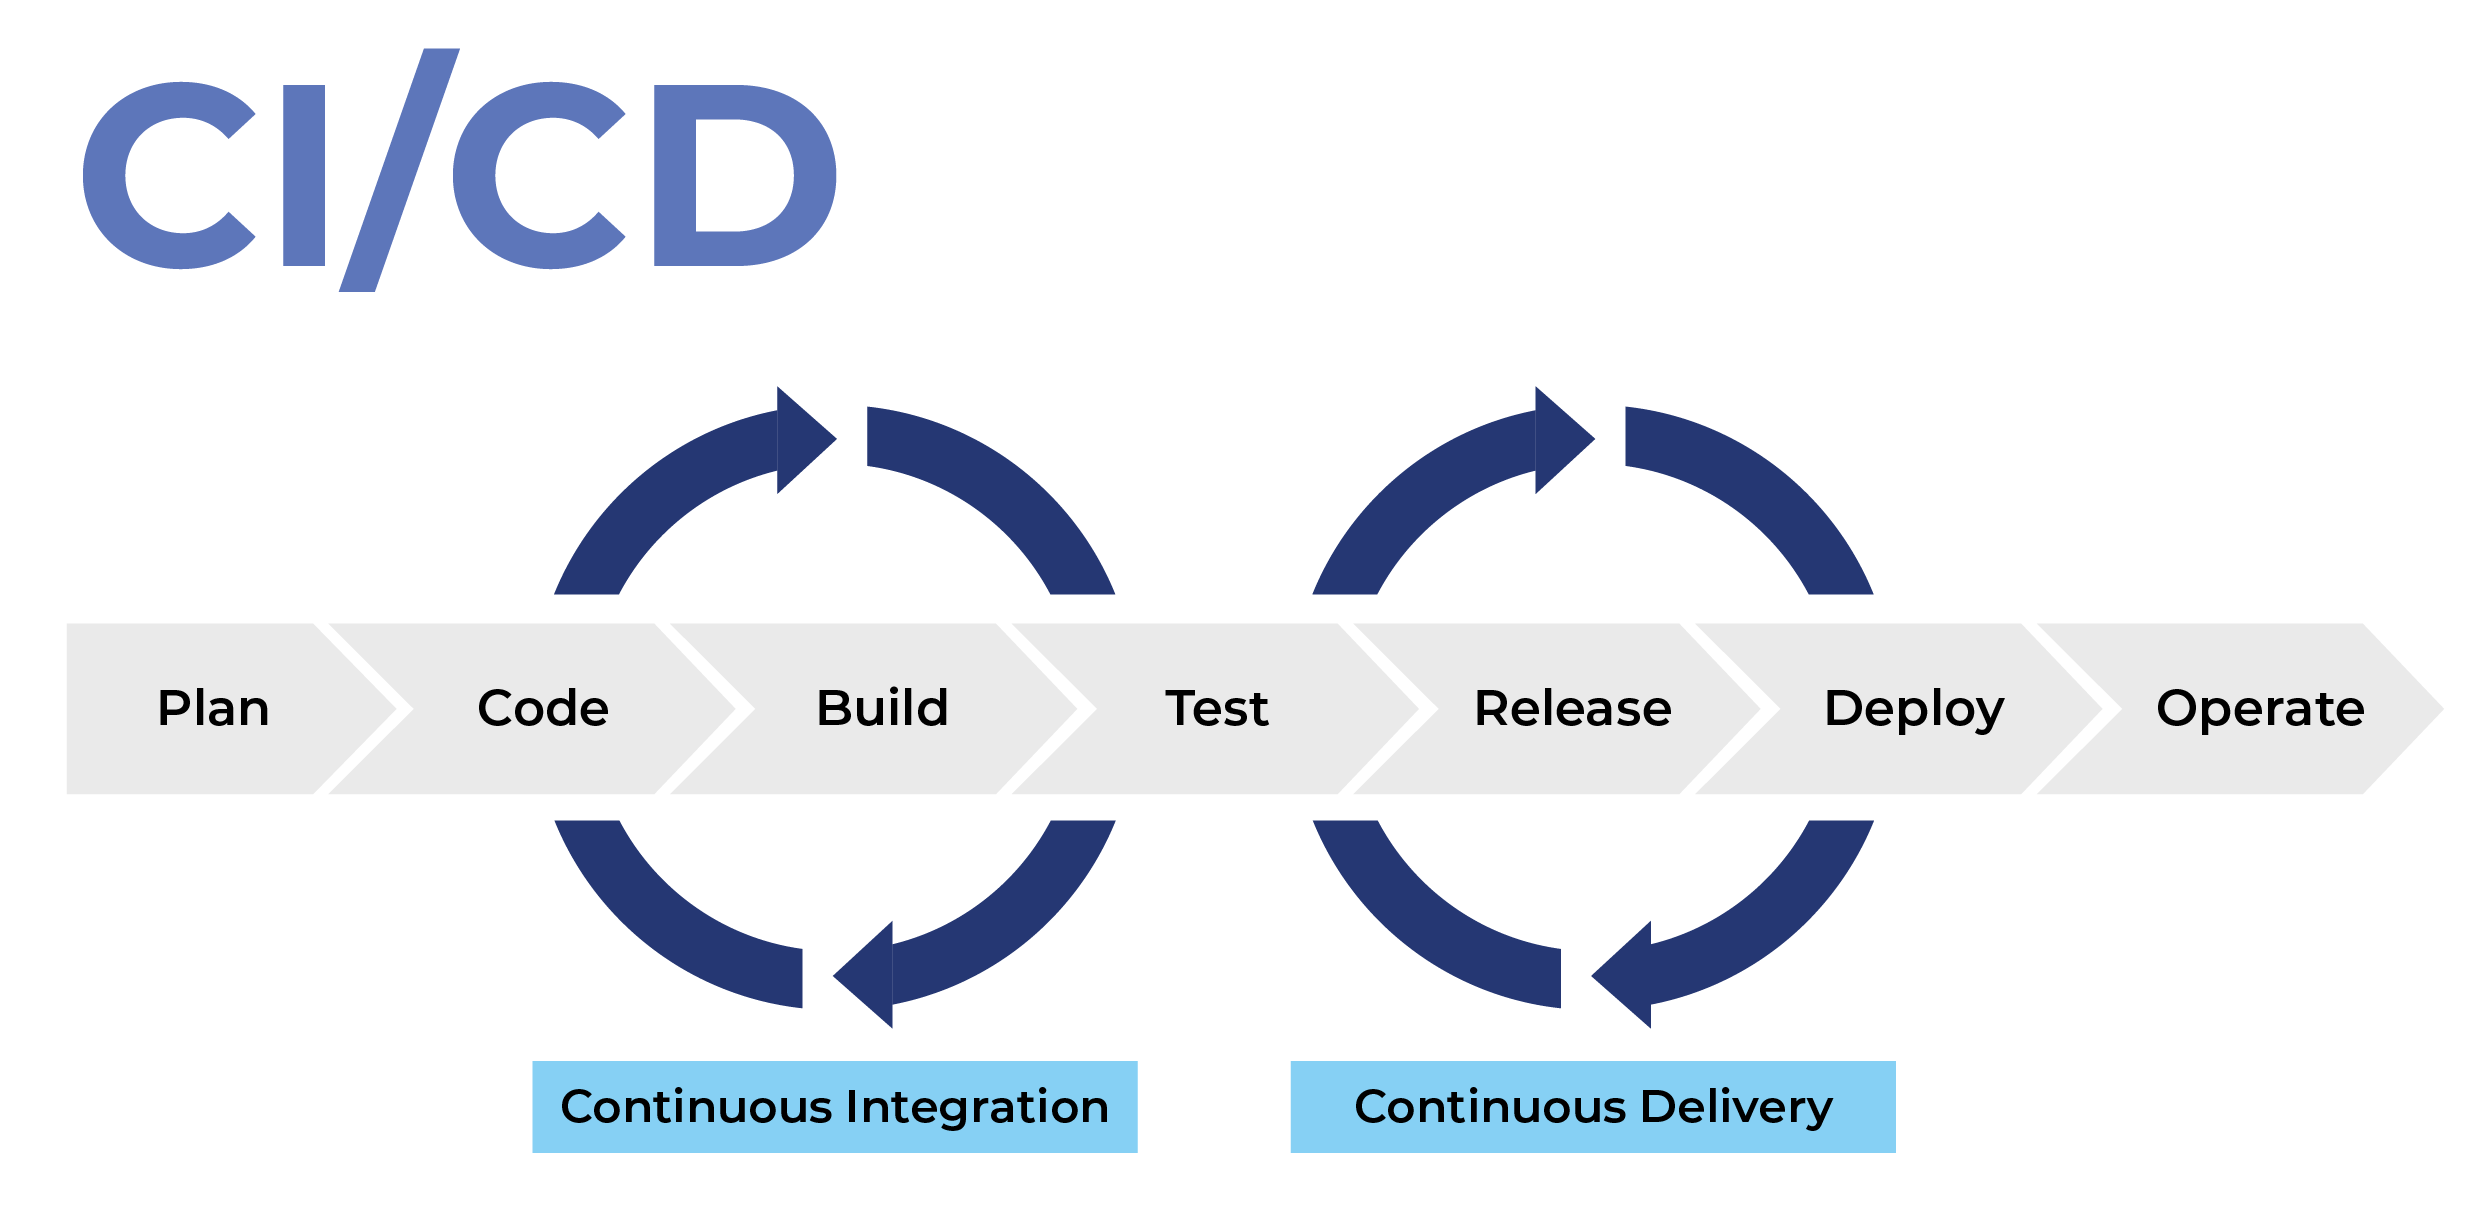
\includegraphics[width=15cm,height=8cm]{Images/Technology/cicd.png}
	\caption[Quy trình CI/CD]{\bfseries \fontsize{12pt}{0pt}
		\selectfont Quy trình CI/CD}
	\label{cicd} %đặt tên cho ảnh
\end{figure}

\subsubsection{Kiến trúc Microservices}
Kiến trúc Microservices là một phương pháp phát triển phần mềm trong đó một
ứng dụng lớn được chia thành nhiều dịch vụ nhỏ độc lập với nhau.  Mỗi dịch vụ thực hiện một chức năng cụ thể và có thể được phát triển, triển khai, mở rộng và bảo trì một cách độc lập với các microservice khác. Chúng thường giao tiếp với nhau thông qua mạng, sử dụng các giao thức như HTTP/REST hoặc message queues.

\begin{figure}[H]
	\centering
	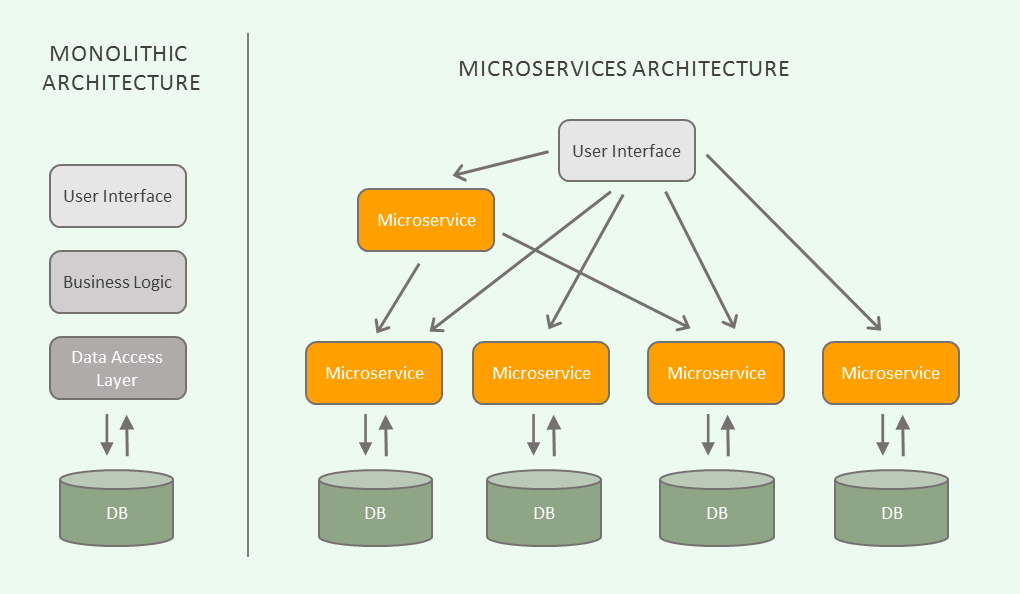
\includegraphics[width=15cm,height=8cm]{Images/Technology/microservice.png}
	\caption[Kiến trúc microservices]{\bfseries \fontsize{12pt}{0pt}
		\selectfont Kiến trúc microservices}
	\label{microservice} %đặt tên cho ảnh
\end{figure}

Một số lợi ích của microservice đã hỗ trợ chúng em:
\begin{itemize}
	\item Tính độc lập: Mỗi microservice là một đơn vị triển khai độc lập. Việc thay đổi một microservice không ảnh hưởng đến các microservice khác, giúp tăng tính linh hoạt và tốc độ phát triển.
	\item Tính chuyên biệt: Mỗi microservice tập trung vào một chức năng nghiệp vụ cụ thể, giúp đơn giản hóa việc phát triển và bảo trì.
	\item Khả năng mở rộng: Có thể mở rộng từng microservice một cách độc lập dựa trên nhu cầu, giúp tối ưu hóa việc sử dụng tài nguyên.
	\item Khả năng chịu lỗi: Nếu một microservice gặp sự cố, các microservice khác vẫn có thể hoạt động bình thường, giúp tăng tính ổn định của hệ thống.
\end{itemize}

% \subsubsection{Triển khai Server và ứng dụng web trên máy chủ VPS}
\subsection{Kiểm thử}

\subsubsection{Kiểm thử hoạt động của các API}


% Môi trường: 

% \begin{adjustwidth}{1.5em}{}
% \begin{itemize}
%   \item Base URL: http://103.200.20.59/ hoặc http://localhost:3000/
% \end{itemize}
% \end{adjustwidth}

Công cụ: Postman - Để xây dựng và thực hiện các yêu cầu API.

\paragraph{API liên quan đến việc xác thực người dùng}
\mbox{}

% Tham khảo bảng \ref{table_api_auth} để xem thông tin của các api liên quan


\begin{enumerate}[a)]
	\item URL: POST auth/register

	      \break
	      \begin{xltabular}{\textwidth}{
		      | >{\raggedright\arraybackslash}p{1cm}
		      | >{\raggedright\arraybackslash}p{2.5cm}
		      | >{\raggedright\arraybackslash}X
		      | >{\raggedright\arraybackslash}X
		      | >{\raggedright\arraybackslash}p{1cm}|
		      }
		      \caption{\bfseries \fontsize{12pt}{0pt}\selectfont Bảng kiểm thử API đăng ký tài khoản}
		      % \label{table_api_news}
		      \\
		      \hline
		      \bfseries Test case    &\bfseries Điều kiện   &\bfseries Đầu vào
		      &\bfseries Mong muốn đầu ra &\bfseries Kết quả\\ \hline


		      TC-1
		      & Người dùng mới
		      & Dữ liệu đăng ký

		      \{

		      "username": "Co Huy Dung",

		      "password": "123456a@",

		      "email": "codung2909@gmail.com",

		      "birth": "29/09/2003",

		      "gender": 1,

		      "phone\_number": "077433306x",

		      "role": 0

		      \}

		      &

		      Status code: 200 OK

		      Response message:

		      \{

		      "status": "success",

		      "message": "register successfully"

		      \}

		      & OK

		      \\ \hline

		      TC-2
		      & Tài khoản email đã tồn tại
		      & Dữ liệu đăng ký

		      \{

		      "username": "Nguyễn Đức B",

		      "password": "xYnF1452",

		      "email": "codung2909@gmail.com",

		      "birth": "15/07/1995",

		      "gender": 1,

		      "phone\_number": "091601736x",

		      "role": 0

		      \}

		      &

		      Status code: 400 Bad Request

		      Response message:

		      \{

		      "status": "error",

		      "message": "email is existed"

		      \}

		      & OK

		      \\ \hline


	      \end{xltabular}


	\item URL: POST auth/login


	      \begin{xltabular}{\textwidth}{
		      | >{\raggedright\arraybackslash}p{1cm}
		      | >{\raggedright\arraybackslash}p{2.5cm}
		      | >{\raggedright\arraybackslash}X
		      | >{\raggedright\arraybackslash}X
		      | >{\raggedright\arraybackslash}p{1cm}|
		      }
		      \caption{\bfseries \fontsize{12pt}{0pt}\selectfont Bảng kiểm thử API người dùng đăng nhập}
		      % \label{table_api_news}
		      \\
		      \hline
		      \bfseries Test case    &\bfseries Điều kiện   &\bfseries Đầu vào
		      &\bfseries Mong muốn đầu ra &\bfseries Kết quả\\ \hline


		      TC-1
		      & Thông tin tài khoản và mật khẩu hợp lệ
		      & Thông tin đăng nhập

		      \{

		      "email": email đã đăng ký,
		      "password": mật khẩu tương ứng

		      \}

		      &

		      Status code: 200 OK

		      Response message:

		      \{

		      "status": "success",

		      data: Thông tin user sau khi đăng ký thành công

		      \}

		      & OK

		      \\ \hline

		      TC-2
		      & Thông tin tài khoản và mật khẩu không hợp lệ
		      & Thông tin đăng nhập

		      \{

		      "email": email người dùng,
		      "password": mật khẩu người dùng

		      \}

		      &

		      Status code: 401 Unauthorized

		      Response message:

		      \{

		      "status": "401 Unauthorized",

		      "message": "Invalid email or password"

		      \}

		      & OK

		      \\ \hline


	      \end{xltabular}



	\item URL: POST auth/logout


	      \begin{xltabular}{\textwidth}{
		      | >{\raggedright\arraybackslash}p{1cm}
		      | >{\raggedright\arraybackslash}p{2.5cm}
		      | >{\raggedright\arraybackslash}X
		      | >{\raggedright\arraybackslash}X
		      | >{\raggedright\arraybackslash}p{1cm}|
		      }
		      \caption{\bfseries \fontsize{12pt}{0pt}\selectfont Bảng kiểm thử API đăng xuất người dùng}
		      % \label{table_api_news}
		      \\
		      \hline
		      \bfseries Test case    &\bfseries Điều kiện   &\bfseries Đầu vào
		      &\bfseries Mong muốn đầu ra &\bfseries Kết quả\\ \hline


		      TC-1
		      & Người dùng đã đăng nhập vào hệ thống
		      & JWT Token tồn tại

		      &

		      Status code: 200 OK

		      Response message:

		      \{

		      "status": "success",

		      "message": "Logged out successfully"

		      \}

		      & OK

		      \\ \hline

		      TC-2
		      & Người dùng chưa đăng nhập vào hệ thống
		      & JWT Token không tồn tại

		      &

		      Status code: 401 Unauthorized

		      Response message:

		      \{

		      "status": "error",

		      "message": "No token found"

		      \}

		      & OK

		      \\ \hline


	      \end{xltabular}



\end{enumerate}



\paragraph{API liên quan đến thông tin người dùng}
\mbox{}

% Tham khảo bảng \ref{table_api_user} để xem thông tin của các api liên quan

\begin{enumerate}[a)]
	\item URL: GET users

	      \begin{xltabular}{\textwidth}{
		      | >{\raggedright\arraybackslash}p{1cm}
		      | >{\raggedright\arraybackslash}p{2.5cm}
		      | >{\raggedright\arraybackslash}p{3.5cm}
		      | >{\raggedright\arraybackslash}X
		      | >{\raggedright\arraybackslash}p{1cm}|
		      }
		      \caption{\bfseries \fontsize{12pt}{0pt}\selectfont Bảng kiểm thử API lấy danh sách người dùng}
		      % \label{table_api_news}
		      \\
		      \hline
		      \bfseries Test case    &\bfseries Điều kiện   &\bfseries Đầu vào
		      &\bfseries Mong muốn đầu ra &\bfseries Kết quả\\ \hline


		      TC-1
		      & Admin của hệ thống
		      & Access token tương ứng

		      &

		      Status code: 200

		      Response message:

		      \{

		      "data": Danh sách người dùng

		      \}

		      & OK

		      \\ \hline

		      TC-2
		      & Không phải admin
		      & Access token tương ứng
		      &

		      Status code: 403

		      Response message:

		      \{

		      "status": "error",

		      "message": "403 Forbidden"

		      \}

		      & OK

		      \\ \hline


		      TC-3
		      & Không có token
		      & NULL

		      &

		      Status code: 401

		      Response message:

		      \{

		      "status": "error",

		      "message": "401 Unauthorized"

		      \}

		      & OK

		      \\ \hline


	      \end{xltabular}

	\item URL: GET users/doctors

	      \begin{xltabular}{\textwidth}{
		      | >{\raggedright\arraybackslash}p{1cm}
		      | >{\raggedright\arraybackslash}p{2.5cm}
		      | >{\raggedright\arraybackslash}p{3.5cm}
		      | >{\raggedright\arraybackslash}X
		      | >{\raggedright\arraybackslash}p{1cm}|
		      }
		      \caption{\bfseries \fontsize{12pt}{0pt}\selectfont Bảng kiểm thử API lấy danh sách bác sĩ}
		      % \label{table_api_news}
		      \\
		      \hline
		      \bfseries Test case    &\bfseries Điều kiện   &\bfseries Đầu vào
		      &\bfseries Mong muốn đầu ra &\bfseries Kết quả\\ \hline


		      TC-1
		      & Admin, bác sĩ của hệ thống
		      & Access token tương ứng

		      &

		      Status code: 200

		      Response message:

		      \{

		      "data": Danh sách bác sĩ

		      \}

		      & OK

		      \\ \hline

		      TC-2
		      & Không phải admin, bác sĩ
		      & Access token tương ứng
		      &

		      Status code: 403

		      Response message:

		      \{

		      "status": "error",

		      "message": "403 Forbidden"

		      \}

		      & OK

		      \\ \hline


		      TC-3
		      & Không có token
		      & NULL

		      &

		      Status code: 401

		      Response message:

		      \{

		      "status": "error",

		      "message": "401 Unauthorized"

		      \}

		      & OK

		      \\ \hline


	      \end{xltabular}

	\item URL: GET users/{:id}

	      \begin{xltabular}{\textwidth}{
		      | >{\raggedright\arraybackslash}p{1cm}
		      | >{\raggedright\arraybackslash}p{2.5cm}
		      | >{\raggedright\arraybackslash}p{2.5cm}
		      | >{\raggedright\arraybackslash}X
		      | >{\raggedright\arraybackslash}p{1cm}|
		      }
		      \caption{\bfseries \fontsize{12pt}{0pt}\selectfont Bảng kiểm thử API lấy dữ liệu người dùng bằng id}
		      \\
		      \hline
		      \bfseries Test case    &\bfseries Điều kiện   &\bfseries Đầu vào
		      &\bfseries Mong muốn đầu ra &\bfseries Kết quả\\ \hline


		      TC-1
		      & Người dùng tồn tại trong hệ thống và có id tương ứng
		      & id người dùng

		      &

		      Status code: 200 OK

		      Response message:

		      \{

		      "data": Thông tin người dùng

		      \}

		      & OK

		      \\ \hline

		      TC-2
		      & Người dùng không tồn tại trong hệ thống với id tương ứng
		      & id người dùng

		      &

		      Status code: 404 Not Found

		      Response message:

		      \{

		      "status": "error",

		      "message": "No user found, please try again"

		      \}

		      & OK

		      \\ \hline


	      \end{xltabular}

	\item URL: GET users/data/patient-data

	      \begin{xltabular}{\textwidth}{
		      | >{\raggedright\arraybackslash}p{1cm}
		      | >{\raggedright\arraybackslash}p{2.5cm}
		      | >{\raggedright\arraybackslash}p{3.5cm}
		      | >{\raggedright\arraybackslash}X
		      | >{\raggedright\arraybackslash}p{1cm}|
		      }
		      \caption{\bfseries \fontsize{12pt}{0pt}\selectfont Bảng kiểm thử API lấy danh sách bệnh nhân theo id của bác sĩ}
		      % \label{table_api_news}
		      \\
		      \hline
		      \bfseries Test case    &\bfseries Điều kiện   &\bfseries Đầu vào
		      &\bfseries Mong muốn đầu ra &\bfseries Kết quả\\ \hline


		      TC-1
		      & Admin, bác sĩ tương ứng với id
		      & id của bác sĩ

		      &

		      Status code: 200

		      Response message:

		      \{

		      "data": Danh sách bệnh nhân

		      \}

		      & OK

		      \\ \hline

		      TC-2
		      & Không phải admin, bác sĩ
		      & id của bác sĩ
		      &

		      Status code: 403

		      Response message:

		      \{

		      "status": "error",

		      "message": "403 Forbidden"

		      \}

		      & OK

		      \\ \hline


		      TC-3
		      & Không có token
		      &

		      &

		      Status code: 401

		      Response message:

		      \{

		      "status": "error",

		      "message": "401 Unauthorized"

		      \}

		      & OK

		      \\ \hline


	      \end{xltabular}

	\item URL: GET users/data/doctor-id

	      \begin{xltabular}{\textwidth}{
		      | >{\raggedright\arraybackslash}p{1cm}
		      | >{\raggedright\arraybackslash}p{2.5cm}
		      | >{\raggedright\arraybackslash}p{3.5cm}
		      | >{\raggedright\arraybackslash}X
		      | >{\raggedright\arraybackslash}p{1cm}|
		      }
		      \caption{\bfseries \fontsize{12pt}{0pt}\selectfont Bảng kiểm thử API lấy danh sách bác sĩ theo id của bệnh nhân}
		      \\
		      \hline
		      \bfseries Test case    &\bfseries Điều kiện   &\bfseries Đầu vào
		      &\bfseries Mong muốn đầu ra &\bfseries Kết quả\\ \hline


		      TC-1
		      & Admin, bác sĩ hoặc bệnh nhân có id tương ứng
		      & id của bệnh nhân

		      &

		      Status code: 200

		      Response message:

		      \{

		      "data": Danh sách bác sĩ của bệnh nhân

		      \}

		      & OK

		      \\ \hline

		      TC-2
		      & Bệnh nhân chưa có bác sĩ
		      & id của bệnh nhân

		      &

		      Status code: 200

		      Response message:

		      \{

		      "status": "error",

		      "message": "No user found, please try again"

		      \}

		      & OK

		      \\ \hline


		      TC-3
		      & Không phải admin, bác sĩ hoặc bệnh nhân
		      & id của bệnh nhân
		      &

		      Status code: 403

		      Response message:

		      \{

		      "status": "error",

		      "message": "403 Forbidden"

		      \}

		      & OK

		      \\ \hline

		      TC-4
		      & Không có token
		      &

		      &

		      Status code: 401

		      Response message:

		      \{

		      "status": "error",

		      "message": "401 Unauthorized"

		      \}

		      & OK

		      \\ \hline


	      \end{xltabular}


	\item URL: PUT users

	      \begin{xltabular}{\textwidth}{
		      | >{\raggedright\arraybackslash}p{1cm}
		      | >{\raggedright\arraybackslash}p{2cm}
		      | >{\raggedright\arraybackslash}X
		      | >{\raggedright\arraybackslash}X
		      | >{\raggedright\arraybackslash}p{1cm}|
		      }
		      \caption{\bfseries \fontsize{12pt}{0pt}\selectfont Bảng kiểm thử API cập nhật thông tin người dùng}
		      \\
		      \hline
		      \bfseries Test case    &\bfseries Điều kiện   &\bfseries Đầu vào
		      &\bfseries Mong muốn đầu ra &\bfseries Kết quả\\ \hline


		      TC-1
		      & Người dùng đã tồn tại trong hệ thống với id cho trước
		      & Dữ liệu cập nhật của người dùng
		      &

		      Status code: 200 OK

		      Response message:

		      \{

		      "data": Dữ liệu người dùng đã được cập nhật

		      \}

		      & OK

		      \\ \hline

		      TC-2
		      & Người dùng không tồn tại trong hệ thống với id cho trước
		      &
		      &

		      Status code: 404 Not found

		      Response message:

		      \{

		      "message": "No user found to update, please try again"

		      \}

		      & OK

		      \\ \hline

		      TC-3
		      & Người dùng không có quyền sửa thông tin
		      &
		      &

		      Status code: 403 Forbidden

		      Response message:

		      \{

		      "message": "403 Forbidden"

		      \}

		      & OK

		      \\ \hline

	      \end{xltabular}


	      % TODO: Note new page
	\item URL: DELETE users/{:userId}

	      \begin{xltabular}{\textwidth}{
		      | >{\raggedright\arraybackslash}p{1cm}
		      | >{\raggedright\arraybackslash}p{2cm}
		      | >{\raggedright\arraybackslash}p{2cm}
		      | >{\raggedright\arraybackslash}X
		      | >{\raggedright\arraybackslash}p{1cm}|
		      }
		      \caption{\bfseries \fontsize{12pt}{0pt}\selectfont Bảng kiểm thử API xóa thông tin người dùng}
		      \\
		      \hline
		      \bfseries Test case    &\bfseries Điều kiện   &\bfseries Đầu vào
		      &\bfseries Mong muốn đầu ra &\bfseries Kết quả\\ \hline


		      TC-1
		      & Người dùng đã tồn tại trong hệ thống với id cho trước
		      & id của người dùng

		      &

		      Status code: 200 OK

		      Response message:

		      \{

		      "message": "User has been deleted successfully"

		      \}

		      & OK

		      \\ \hline

		      TC-2
		      & Người dùng không tồn tại trong hệ thống với id cho trước
		      & id của người dùng

		      &

		      Status code: 404 Not found

		      Response message:

		      \{

		      "message": "No user found to delete, please try again"

		      \}

		      & OK
		      \\ \hline

	      \end{xltabular}

	\item URL: GET statistic

	      \begin{xltabular}{\textwidth}{
		      | >{\raggedright\arraybackslash}p{1cm}
		      | >{\raggedright\arraybackslash}p{2cm}
		      | >{\raggedright\arraybackslash}p{2cm}
		      | >{\raggedright\arraybackslash}X
		      | >{\raggedright\arraybackslash}p{1cm}|
		      }
		      \caption{\bfseries \fontsize{12pt}{0pt}\selectfont Bảng kiểm thử API lấy dữ liệu thống kê}
		      \\
		      \hline
		      \bfseries Test case    &\bfseries Điều kiện   &\bfseries Đầu vào
		      &\bfseries Mong muốn đầu ra &\bfseries Kết quả\\ \hline


		      TC-1
		      & Admin của hệ thống
		      & Access token tương ứng

		      &

		      Status code: 200 OK

		      Response message:

		      \{

		      data: dữ liệu thống kê số lượng người dùng, thiết bị, dữ liệu phiên đo mỗi tháng

		      \}

		      & OK

		      \\ \hline

		      TC-2
		      & Không phải admin của hệ thống
		      & Access token tương ứng

		      &

		      Status code: 403 Forbidden

		      Response message:

		      \{

		      "message": "403 Forbidden"

		      \}

		      & OK
		      \\ \hline

	      \end{xltabular}


\end{enumerate}


\paragraph{API liên quan đến thiết bị}
\mbox{}

% Tham khảo bảng \ref{table_api_device} để xem thông tin của các api liên quan

\begin{enumerate}[a)]
	\item URL: GET device

	      \begin{xltabular}{\textwidth}{
		      | >{\raggedright\arraybackslash}p{1cm}
		      | >{\raggedright\arraybackslash}p{2.5cm}
		      | >{\raggedright\arraybackslash}p{2.5cm}
		      | >{\raggedright\arraybackslash}X
		      | >{\raggedright\arraybackslash}p{1cm}|
		      }
		      \caption{\bfseries \fontsize{12pt}{0pt}\selectfont Bảng kiểm thử API lấy danh sách thiết bị}
		      % \label{table_api_news}
		      \\
		      \hline
		      \bfseries Test case    &\bfseries Điều kiện   &\bfseries Đầu vào
		      &\bfseries Mong muốn đầu ra &\bfseries Kết quả\\ \hline


		      TC-1
		      & Admin của hệ thống
		      & Access token tương ứng
		      &

		      Status code: 200 OK

		      Response message:

		      \{

		      "data": Danh sách thiết bị

		      \}
		      & OK

		      \\ \hline

		      TC-2
		      & Không phải admin của hệ thống
		      & Access token tương ứng

		      &

		      Status code: 403 Forbidden

		      Response message:

		      \{

		      "message": "403 Forbidden"

		      \}
		      & OK
		      \\ \hline


	      \end{xltabular}


	\item URL: GET device/{:id}

	      \begin{xltabular}{\textwidth}{
		      | >{\raggedright\arraybackslash}p{1cm}
		      | >{\raggedright\arraybackslash}p{2.5cm}
		      | >{\raggedright\arraybackslash}p{2.5cm}
		      | >{\raggedright\arraybackslash}X
		      | >{\raggedright\arraybackslash}p{1cm}|
		      }
		      \caption{\bfseries \fontsize{12pt}{0pt}\selectfont Bảng kiểm thử API lấy dữ liệu thiết bị theo id}
		      % \label{table_api_news}
		      \\
		      \hline
		      \bfseries Test case    &\bfseries Điều kiện   &\bfseries Đầu vào
		      &\bfseries Mong muốn đầu ra &\bfseries Kết quả\\ \hline


		      TC-1
		      & Thiết bị tồn tại với id cho trước
		      & id thiết bị
		      &

		      Status code: 200 OK

		      Response message:

		      \{

		      data: Thông tin của thiết bị

		      \}
		      & OK

		      \\ \hline

		      TC-2
		      & Thiết bị không tồn tại với id cho trước
		      & id thiết bị
		      &

		      Status code: 404 Not Found

		      Response message:

		      \{

		      "message": "No device found, please try again"

		      \}
		      & OK

		      \\ \hline


	      \end{xltabular}

	      % //TODO: new page
	\item URL: POST device/add

	      \begin{xltabular}{\textwidth}{
		      | >{\raggedright\arraybackslash}p{1cm}
		      | >{\raggedright\arraybackslash}p{2.5cm}
		      | >{\raggedright\arraybackslash}X
		      | >{\raggedright\arraybackslash}X
		      | >{\raggedright\arraybackslash}p{1cm}|
		      }
		      \caption{\bfseries \fontsize{12pt}{0pt}\selectfont Bảng kiểm thử API thêm thiết bị}
		      % \label{table_api_news}
		      \\
		      \hline
		      \bfseries Test case    &\bfseries Điều kiện   &\bfseries Đầu vào
		      &\bfseries Mong muốn đầu ra &\bfseries Kết quả\\ \hline


		      TC-1
		      & Bệnh nhân và bác sĩ tồn tại với ID tương ứng
		      & Thông tin thiết bị

		      \{

		      "user\_id": id bệnh nhân,

		      "device\_name": Tên thiết bị,

		      "infomation": Thông tin thiết bị,

		      "device\_type\_id": id loại thiết bị,

		      "status\_id": id trạng thái thiết bị,

		      "start\_time": Giờ bắt đầu sử dụng

		      "end\_time": Giờ kết thúc sử dụng

		      \}
		      &

		      Status code: 200 OK

		      Response message:

		      \{
		      "message": "Device created successfully",

		      data: Thông tin của thiết bị

		      \}

		      & OK

		      \\ \hline

		      TC-2
		      & Người dùng không tồn tại với id đã cho
		      & Thông tin thiết bị

		      \{

		      "user\_id": id bệnh nhân,

		      "device\_name": Tên thiết bị,

		      "infomation": Thông tin thiết bị,

		      "device\_type\_id": id loại thiết bị,

		      "status\_id": id trạng thái thiết bị,

		      "start\_time": Giờ bắt đầu sử dụng

		      "end\_time": Giờ kết thúc sử dụng

		      \}
		      &

		      Status code: 404 Not found

		      Response message:

		      \{

		      "message": "No user found, please try again"

		      \}

		      & OK

		      \\ \hline


	      \end{xltabular}

	\item URL: POST device\_detail
	      \begin{xltabular}{\textwidth}{
		      | >{\raggedright\arraybackslash}p{1cm}
		      | >{\raggedright\arraybackslash}p{2.5cm}
		      | >{\raggedright\arraybackslash}X
		      | >{\raggedright\arraybackslash}X
		      | >{\raggedright\arraybackslash}p{1cm}|
		      }
		      \caption{\bfseries \fontsize{12pt}{0pt}\selectfont Bảng kiểm thử API thêm chi tiết thông tin thiết bị}
		      % \label{table_api_news}
		      \\
		      \hline
		      \bfseries Test case    &\bfseries Điều kiện   &\bfseries Đầu vào
		      &\bfseries Mong muốn đầu ra &\bfseries Kết quả\\ \hline


		      TC-1
		      & Thiết bị tồn tại với id cho trước
		      & Chi tiết thông tin thiết bị

		      \{

		      "device\_id": id thiết bị,

		      "detail\_name": Tên chi tiết,

		      "detail\_type": loại chi tiết,

		      "value": giá trị,

		      "infomation": Thông tin ghi chú chi tiết,

		      \}
		      &

		      Status code: 200 OK

		      Response message:

		      \{

		      "message": "Device detail created successfully",

		      data: Chi tiết thông tin của thiết bị

		      \}

		      & OK

		      \\ \hline

		      TC-2
		      & Thiết bị không tồn tại với id cho trước
		      & Chi tiết thông tin thiết bị

		      \{

		      "device\_id": id thiết bị,

		      "detail\_name": Tên chi tiết,

		      "detail\_type": loại chi tiết,

		      "value": giá trị,

		      "infomation": Thông tin ghi chú chi tiết,

		      \}
		      &

		      Status code: 404 Not found

		      Response message:

		      \{

		      "message": "Device not found"

		      \}

		      & OK

		      \\ \hline

		      TC-3
		      & Người dùng không tồn tại với id tương ứng
		      & Chi tiết thông tin thiết bị

		      \{

		      "device\_id": id thiết bị,

		      "detail\_name": Tên chi tiết,

		      "detail\_type": loại chi tiết,

		      "value": giá trị,

		      "infomation": Thông tin ghi chú chi tiết,

		      \}
		      &

		      Status code: 404 Not found

		      Response message:

		      \{

		      "message": "No user found, please try again"

		      \}

		      & OK

		      \\ \hline

	      \end{xltabular}

	\item URL: DELETE device/{:device\_id}

	      \begin{xltabular}{\textwidth}{
		      | >{\raggedright\arraybackslash}p{1cm}
		      | >{\raggedright\arraybackslash}p{2.5cm}
		      | >{\raggedright\arraybackslash}p{2.5cm}
		      | >{\raggedright\arraybackslash}X
		      | >{\raggedright\arraybackslash}p{1cm}|
		      }
		      \caption{\bfseries \fontsize{12pt}{0pt}\selectfont Bảng kiểm thử API xóa thiết bị theo id}
		      % \label{table_api_news}
		      \\
		      \hline
		      \bfseries Test case    &\bfseries Điều kiện   &\bfseries Đầu vào
		      &\bfseries Mong muốn đầu ra &\bfseries Kết quả\\ \hline


		      TC-1
		      & Thiết bị tồn tại với id cho trước
		      & id thiết bị

		      &

		      Status code: 200 OK

		      Response message:

		      \{

		      "message": "Delete device successful"

		      \}

		      & OK

		      \\ \hline

		      TC-2
		      & Không tồn tại thiết bị với id cho trước
		      & id thiết bị

		      &

		      Status code: 404 Not found

		      Response message:

		      \{

		      "message": "Device not found"

		      \}

		      & OK

		      \\ \hline


	      \end{xltabular}

	\item URL: PUT device/{:device\_id}
	      \begin{xltabular}{\textwidth}{
		      | >{\raggedright\arraybackslash}p{1cm}
		      | >{\raggedright\arraybackslash}p{2.5cm}
		      | >{\raggedright\arraybackslash}X
		      | >{\raggedright\arraybackslash}X
		      | >{\raggedright\arraybackslash}p{1cm}|
		      }
		      \caption{\bfseries \fontsize{12pt}{0pt}\selectfont Bảng kiểm thử API cập nhật thông tin thiết bị}
		      % \label{table_api_news}
		      \\
		      \hline
		      \bfseries Test case    &\bfseries Điều kiện   &\bfseries Đầu vào
		      &\bfseries Đầu ra mong muốn &\bfseries Kết quả\\ \hline


		      TC-1
		      & Thiết bị tồn tại với id cho trước
		      & Thông tin thiết bị

		      \{

		      "user\_id": id bệnh nhân,

		      "device\_name": Tên thiết bị,

		      "infomation": Thông tin thiết bị,

		      "device\_type\_id": id loại thiết bị,

		      "status\_id": id trạng thái thiết bị,

		      "start\_time": Giờ bắt đầu sử dụng

		      "end\_time": Giờ kết thúc sử dụng

		      \}
		      &

		      Status code: 200 OK

		      Response content:

		      \{

		      data: Thông tin sau khi cập nhật của thiết bị

		      \}

		      & OK

		      \\ \hline

		      TC-2
		      & Không tồn tại thiết bị với id cho trước
		      & Thông tin thiết bị

		      \{

		      "user\_id": id bệnh nhân,

		      "device\_name": Tên thiết bị,

		      "infomation": Thông tin thiết bị,

		      "device\_type\_id": id loại thiết bị,

		      "status\_id": id trạng thái thiết bị,

		      "start\_time": Giờ bắt đầu sử dụng

		      "end\_time": Giờ kết thúc sử dụng

		      \}
		      &

		      Status code: 404 Not found

		      Response content:

		      \{

		      "message": "No device found to update, please try again"

		      \}

		      & OK

		      \\ \hline

		      TC-3
		      & Người dùng không tồn tại với id cho trước
		      & Thông tin thiết bị

		      \{

		      "user\_id": id bệnh nhân,

		      "device\_name": Tên thiết bị,

		      "infomation": Thông tin thiết bị,

		      "device\_type\_id": id loại thiết bị,

		      "status\_id": id trạng thái thiết bị,

		      "start\_time": Giờ bắt đầu sử dụng

		      "end\_time": Giờ kết thúc sử dụng

		      \}
		      &

		      Status code: 404 Not found

		      Response content:

		      \{

		      "message": "No user found, please try again"

		      \}

		      & OK

		      \\ \hline

	      \end{xltabular}

	\item URL: PUT device\_detail/
	      \begin{xltabular}{\textwidth}{
		      | >{\raggedright\arraybackslash}p{1cm}
		      | >{\raggedright\arraybackslash}p{2.5cm}
		      | >{\raggedright\arraybackslash}X
		      | >{\raggedright\arraybackslash}X
		      | >{\raggedright\arraybackslash}p{1cm}|
		      }
		      \caption{\bfseries \fontsize{12pt}{0pt}\selectfont Bảng kiểm thử API cập nhật chi tiết thông tin thiết bị}
		      % \label{table_api_news}
		      \\
		      \hline
		      \bfseries Test case    &\bfseries Điều kiện   &\bfseries Đầu vào
		      &\bfseries Mong muốn đầu ra &\bfseries Kết quả\\ \hline


		      TC-1
		      & Thông tin chi tiết mới phù hợp
		      & Chi tiết thông tin thiết bị

		      \{

		      "device\_id": id thiết bị,

		      "detail\_name": Tên chi tiết,

		      "detail\_type": loại chi tiết,

		      "value": giá trị,

		      "infomation": Thông tin ghi chú chi tiết,

		      \}
		      &

		      Status code: 200 OK

		      Response message:

		      \{

		      "message": "Device detail updated successfully",

		      data: Chi tiết thông tin của thiết bị sau khi cập nhật

		      \}

		      & OK

		      \\ \hline

		      TC-2
		      & Thông tin chi tiết mới không phù hợp
		      & Chi tiết thông tin thiết bị

		      \{

		      "device\_id": id thiết bị,

		      "detail\_name": Tên chi tiết,

		      "detail\_type": loại chi tiết,

		      "value": giá trị,

		      "infomation": Thông tin ghi chú chi tiết,

		      \}
		      &

		      Status code: 400 Bad Request

		      Response message:

		      \{

		      "message": "Error when update device"

		      \}

		      & OK

		      \\ \hline
	      \end{xltabular}

	\item URL: DELETE device\_detail/{:detail\_id}
	      \begin{xltabular}{\textwidth}{
		      | >{\raggedright\arraybackslash}p{1cm}
		      | >{\raggedright\arraybackslash}p{2.5cm}
		      | >{\raggedright\arraybackslash}X
		      | >{\raggedright\arraybackslash}X
		      | >{\raggedright\arraybackslash}p{1cm}|
		      }
		      \caption{\bfseries \fontsize{12pt}{0pt}\selectfont Bảng kiểm thử API xóa chi tiết thông tin thiết bị}
		      % \label{table_api_news}
		      \\
		      \hline
		      \bfseries Test case    &\bfseries Điều kiện   &\bfseries Đầu vào
		      &\bfseries Mong muốn đầu ra &\bfseries Kết quả\\ \hline


		      TC-1
		      & Thông tin chi tiết mới phù hợp
		      & id chi tiết thông tin thiết bị
		      &

		      Status code: 200 OK

		      Response message:

		      \{

		      "message": "Device detail deleted successfully",

		      data: Chi tiết thông tin của thiết bị sau khi cập nhật

		      \}

		      & OK

		      \\ \hline
	      \end{xltabular}
\end{enumerate}



\paragraph{API liên quan đến dữ liệu phiên đo}
\mbox{}

\begin{enumerate}[a)]
	\item URL: GET records
	      \begin{xltabular}{\textwidth}{
		      | >{\raggedright\arraybackslash}p{1cm}
		      | >{\raggedright\arraybackslash}p{2.5cm}
		      | >{\raggedright\arraybackslash}p{2.5cm}
		      | >{\raggedright\arraybackslash}X
		      | >{\raggedright\arraybackslash}p{1cm}|
		      }
		      \caption{\bfseries \fontsize{12pt}{0pt}\selectfont Bảng kiểm thử API lấy tất cả dữ liệu phiên đo}
		      % \label{table_api_news}
		      \\
		      \hline
		      \bfseries Test case    &\bfseries Điều kiện   &\bfseries Đầu vào
		      &\bfseries Mong muốn đầu ra &\bfseries Kết quả\\ \hline


		      TC-1
		      & Admin của hệ thống
		      & Access Token tương ứng

		      &

		      Status code: 200 OK

		      Response message:

		      \{

		      data: Danh sách dữ liệu phiên đo

		      \}

		      & OK

		      \\ \hline

		      TC-2
		      & Không phải admin của hệ thống
		      & Access Token tương ứng

		      &

		      Status code: 403 Forbidden

		      Response message:

		      \{

		      "message": "Forbidden"

		      \}

		      & OK
		      \\ \hline


	      \end{xltabular}

	\item URL: GET records/{:id}
	      \begin{xltabular}{\textwidth}{
		      | >{\raggedright\arraybackslash}p{1cm}
		      | >{\raggedright\arraybackslash}p{2.5cm}
		      | >{\raggedright\arraybackslash}p{2.5cm}
		      | >{\raggedright\arraybackslash}X
		      | >{\raggedright\arraybackslash}p{1cm}|
		      }
		      \caption{\bfseries \fontsize{12pt}{0pt}\selectfont Bảng kiểm thử API lấy dữ liệu phiên đo theo id}
		      % \label{table_api_news}
		      \\
		      \hline
		      \bfseries Test case    &\bfseries Điều kiện   &\bfseries Đầu vào
		      &\bfseries Mong muốn đầu ra &\bfseries Kết quả\\ \hline


		      TC-1
		      & Là admin, bác sĩ của hệ thống, dữ liệu phiên đo tồn tại
		      & id của dữ liệu phiên đo

		      &

		      Status code: 200 OK

		      Response message:

		      \{

		      "data": Danh sách tất cả dữ liệu phiên đo trong hệ thống

		      \}
		      & OK

		      \\ \hline

		      TC-2
		      & Không phải admin, bác sĩ
		      & id của dữ liệu phiên đo

		      &

		      Status code: 403 Forbidden

		      Response message:

		      \{

		      "message": "Forbidden"

		      \}
		      & OK

		      \\ \hline

		      TC-3
		      & Là admin, bác sĩ của hệ thống, dữ liệu phiên đo không tồn tại
		      & id của dữ liệu phiên đo

		      &

		      Status code: 404 Not Found

		      Response message:

		      \{

		      "message": "No record found, please try again"

		      \}
		      & OK

		      \\ \hline


	      \end{xltabular}


	\item URL: GET records/doctor/{:doctorId}
	      \begin{xltabular}{\textwidth}{
		      | >{\raggedright\arraybackslash}p{1cm}
		      | >{\raggedright\arraybackslash}p{2.5cm}
		      | >{\raggedright\arraybackslash}p{2.5cm}
		      | >{\raggedright\arraybackslash}X
		      | >{\raggedright\arraybackslash}p{1cm}|
		      }
		      \caption{\bfseries \fontsize{12pt}{0pt}\selectfont Bảng kiểm thử API lấy các dữ liệu phiên đo theo id của bác sĩ}
		      % \label{table_api_news}
		      \\
		      \hline
		      \bfseries Test case    &\bfseries Điều kiện   &\bfseries Đầu vào
		      &\bfseries Mong muốn đầu ra &\bfseries Kết quả\\ \hline


		      TC-1
		      & Là admin hoặc bác sĩ có id cho trước
		      & id bác sĩ

		      &

		      Status code: 200 OK

		      Response message:

		      \{

		      data: Danh sách các dữ liệu phiên đo của bác sĩ

		      \}
		      & OK
		      \\ \hline

		      TC-2
		      & Không phải là admin hoặc bác sĩ tương ứng
		      & id bác sĩ

		      &

		      Status code: 403 Forbidden

		      Response message:

		      \{

		      "message": "Forbidden"

		      \}
		      & OK
		      \\ \hline


	      \end{xltabular}

	\item URL: POST records
	      \begin{xltabular}{\textwidth}{
		      | >{\raggedright\arraybackslash}p{1cm}
		      | >{\raggedright\arraybackslash}p{2.5cm}
		      | >{\raggedright\arraybackslash}X
		      | >{\raggedright\arraybackslash}X
		      | >{\raggedright\arraybackslash}p{1cm}|
		      }
		      \caption{\bfseries \fontsize{12pt}{0pt}\selectfont Bảng kiểm thử API thêm dữ liệu phiên đo}
		      % \label{table_api_news}
		      \\
		      \hline
		      \bfseries Test case    &\bfseries Điều kiện   &\bfseries Đầu vào
		      &\bfseries Mong muốn đầu ra &\bfseries Kết quả\\ \hline


		      TC-1
		      & Là admin hoặc bác sĩ, file hợp lệ,
		      & Thông tin dữ liệu phiên đo

		      \{

		      "patient\_id": ID bệnh nhân,

		      "device\_id": ID thiết bị,

		      "record\_type": Loại dữ liệu phiên đo,

		      "start\_time": Thời gian bắt đầu,

		      "end\_time": Thời gian kết thúc,

		      "data\_rec\_url": Đường dẫn file dữ liệu phiên đo

		      \}
		      &

		      Status code: 200 OK

		      Response message:

		      \{

		      "message": "Record created successfully"

		      \}
		      & OK

		      \\ \hline

		      TC-2
		      & Là admin hoặc bác sĩ, file không hợp lệ,
		      & Thông tin dữ liệu phiên đo

		      \{

		      "patient\_id": ID bệnh nhân,

		      "device\_id": ID thiết bị,

		      "record\_type": Loại dữ liệu phiên đo,

		      "start\_time": Thời gian bắt đầu,

		      "end\_time": Thời gian kết thúc,

		      "data\_rec\_url": Đường dẫn file dữ liệu phiên đo

		      \}
		      &

		      Status code: 400 Bad Request

		      Response message:

		      \{

		      "message": "Invalid file type"

		      \}
		      & OK

		      \\ \hline

		      TC-3
		      & Thông tin dữ liệu phiên đo không hợp lệ
		      & Thông tin dữ liệu phiên đo

		      \{

		      "patient\_id": ID bệnh nhân,

		      "device\_id": ID thiết bị,

		      "record\_type": Loại dữ liệu phiên đo,

		      "start\_time": Thời gian bắt đầu,

		      "end\_time": Thời gian kết thúc,

		      "data\_rec\_url": Đường dẫn file dữ liệu phiên đo

		      \}
		      &

		      Status code: 400 Bad Request

		      Response message:

		      \{

		      "message": "Failed to create record"

		      \}
		      & OK

		      \\ \hline

	      \end{xltabular}

	\item URL: PUT records
	      \begin{xltabular}{\textwidth}{
		      | >{\raggedright\arraybackslash}p{1cm}
		      | >{\raggedright\arraybackslash}p{2cm}
		      | >{\raggedright\arraybackslash}X
		      | >{\raggedright\arraybackslash}X
		      | >{\raggedright\arraybackslash}p{1cm}|
		      }
		      \caption{\bfseries \fontsize{12pt}{0pt}\selectfont Bảng kiểm thử API cập nhật dữ liệu dữ liệu phiên đo}
		      % \label{table_api_news}
		      \\
		      \hline
		      \bfseries Test case    &\bfseries Điều kiện   &\bfseries Đầu vào
		      &\bfseries Mong muốn đầu ra &\bfseries Kết quả\\ \hline


		      TC-1
		      & Dữ liệu cập nhật phù hợp
		      & Thông tin cập nhật dữ liệu phiên đo
		      \{

		      "patient\_id": ID bệnh nhân,

		      "device\_id": ID thiết bị,

		      "record\_type": Loại dữ liệu phiên đo,

		      "start\_time": Thời gian bắt đầu,

		      "end\_time": Thời gian kết thúc,

		      "data\_rec\_url": Đường dẫn file dữ liệu phiên đo

		      \}
		      &

		      Status code: 200 OK

		      Response message:

		      \{

		      "message": "Record updated successfully"

		      \}

		      & OK

		      \\ \hline

		      TC-2
		      & Dữ liệu cập nhật không phù hợp
		      & Thông tin cập nhật dữ liệu phiên đo
		      \{

		      "patient\_id": ID bệnh nhân,

		      "device\_id": ID thiết bị,

		      "record\_type": Loại dữ liệu phiên đo,

		      "start\_time": Thời gian bắt đầu,

		      "end\_time": Thời gian kết thúc,

		      "data\_rec\_url": Đường dẫn file dữ liệu phiên đo

		      \}

		      &

		      Status code: 404 Not Found

		      Response message:

		      \{

		      "message": "Error when update record"

		      \}

		      & OK

		      \\ \hline
	      \end{xltabular}

	\item URL: DELETE records/{:record\_id}
	      \begin{xltabular}{\textwidth}{
		      | >{\raggedright\arraybackslash}p{1cm}
		      | >{\raggedright\arraybackslash}p{2.5cm}
		      | >{\raggedright\arraybackslash}p{2.5cm}
		      | >{\raggedright\arraybackslash}X
		      | >{\raggedright\arraybackslash}p{1cm}|
		      }
		      \caption{\bfseries \fontsize{12pt}{0pt}\selectfont Bảng kiểm thử API xóa dữ liệu dữ liệu phiên đo theo id}
		      % \label{table_api_news}
		      \\
		      \hline
		      \bfseries Test case    &\bfseries Điều kiện   &\bfseries Đầu vào
		      &\bfseries Mong muốn đầu ra &\bfseries Kết quả\\ \hline


		      TC-1
		      & Tồn tại dữ liệu phiên đo với id cho trước
		      & id dữ liệu phiên đo

		      &

		      Status code: 200 OK

		      Response message:

		      \{

		      "message": "Record deleted successfully"

		      \}
		      & OK

		      \\ \hline

		      TC-2
		      & Không tồn tại dữ liệu phiên đo với id cho trước
		      & id dữ liệu phiên đo

		      &

		      Status code: 404 Not Found

		      Response message:

		      \{

		      "message": "No record found to delete, please try again"

		      \}
		      & OK

		      \\ \hline


	      \end{xltabular}


\end{enumerate}


\paragraph{API liên quan liên quan đến việc đặt lịch bác sĩ - bệnh nhân}
\mbox{}

\begin{enumerate}[a)]
	\item URL: GET schedules
	      \begin{xltabular}{\textwidth}{
		      | >{\raggedright\arraybackslash}p{1cm}
		      | >{\raggedright\arraybackslash}p{2.5cm}
		      | >{\raggedright\arraybackslash}p{2.5cm}
		      | >{\raggedright\arraybackslash}X
		      | >{\raggedright\arraybackslash}p{1cm}|
		      }
		      \caption{\bfseries \fontsize{12pt}{0pt}\selectfont Bảng kiểm thử API lấy tất cả lịch hẹn của các bác sĩ - các bệnh nhân}
		      % \label{table_api_news}
		      \\
		      \hline
		      \bfseries Test case    &\bfseries Điều kiện   &\bfseries Đầu vào
		      &\bfseries Mong muốn đầu ra &\bfseries Kết quả\\ \hline


		      TC-1
		      & Admin hệ thống
		      & Access token tương ứng
		      &

		      Status code: 200 OK

		      Response message:

		      \{

		      data: Danh sách tất cả lịch hẹn

		      \}
		      & OK

		      \\ \hline

		      TC-2
		      & Không phải admin hệ thống
		      & NULL

		      &

		      Status code: 403 Forbidden

		      Response message:

		      \{

		      "message": "Forbidden"

		      \}
		      & OK
		      \\ \hline
	      \end{xltabular}

	\item URL: GET schedules/doctor-id
	      \begin{xltabular}{\textwidth}{
		      | >{\raggedright\arraybackslash}p{1cm}
		      | >{\raggedright\arraybackslash}p{2.5cm}
		      | >{\raggedright\arraybackslash}X
		      | >{\raggedright\arraybackslash}X
		      | >{\raggedright\arraybackslash}p{1cm}|
		      }
		      \caption{\bfseries \fontsize{12pt}{0pt}\selectfont Bảng kiểm thử API lấy danh sách lịch hẹn theo id bác sĩ}
		      % \label{table_api_news}
		      \\
		      \hline
		      \bfseries Test case    &\bfseries Điều kiện   &\bfseries Đầu vào
		      &\bfseries Mong muốn đầu ra &\bfseries Kết quả\\ \hline


		      TC-1
		      & Bác sĩ tồn tại trong hệ thống
		      & id bác sĩ
		      &

		      Status code: 200 OK

		      Response message:

		      \{

		      data: Danh sách lịch hẹn của bác sĩ

		      \}

		      & OK

		      \\ \hline

		      TC-2
		      & Bác sĩ không tồn tại trong hệ thống
		      & id bác sĩ
		      &

		      Status code: 404 Not Found

		      Response message:

		      \{

		      "status": "error",

		      "message": "No user found, please try again."

		      \}

		      & OK

		      \\ \hline


	      \end{xltabular}

	\item URL: GET schedules/patient-id
	      \begin{xltabular}{\textwidth}{
		      | >{\raggedright\arraybackslash}p{1cm}
		      | >{\raggedright\arraybackslash}p{2.5cm}
		      | >{\raggedright\arraybackslash}X
		      | >{\raggedright\arraybackslash}X
		      | >{\raggedright\arraybackslash}p{1cm}|
		      }
		      \caption{\bfseries \fontsize{12pt}{0pt}\selectfont Bảng kiểm thử API lấy danh sách lịch hẹn theo id bệnh nhân}
		      % \label{table_api_news}
		      \\
		      \hline
		      \bfseries Test case    &\bfseries Điều kiện   &\bfseries Đầu vào
		      &\bfseries Mong muốn đầu ra &\bfseries Kết quả\\ \hline


		      TC-1
		      & Bệnh nhân tồn tại trong hệ thống
		      & id bác sĩ
		      &

		      Status code: 200 OK

		      Response message:

		      \{

		      data: Danh sách lịch hẹn của bệnh nhân

		      \}

		      & OK

		      \\ \hline

		      TC-2
		      & Bệnh nhân không tồn tại trong hệ thống
		      & id bác sĩ
		      &

		      Status code: 404 Not Found

		      Response message:

		      \{

		      "status": "error",

		      "message": "No user found, please try again."

		      \}

		      & OK

		      \\ \hline


	      \end{xltabular}

	\item URL: POST schedules/create-by-doctor
	      \begin{xltabular}{\textwidth}{
		      | >{\raggedright\arraybackslash}p{1cm}
		      | >{\raggedright\arraybackslash}p{2cm}
		      | >{\raggedright\arraybackslash}X
		      | >{\raggedright\arraybackslash}X
		      | >{\raggedright\arraybackslash}p{1cm}|
		      }
		      \caption{\bfseries \fontsize{12pt}{0pt}\selectfont Bảng kiểm thử API tạo lịch hẹn bởi bác sĩ}
		      % \label{table_api_news}
		      \\
		      \hline
		      \bfseries Test case    &\bfseries Điều kiện   &\bfseries Đầu vào
		      &\bfseries Mong muốn đầu ra &\bfseries Kết quả\\ \hline


		      TC-1
		      & Các trường thông tin lịch hẹn hợp lệ
		      & Thông tin lịch hẹn
		      \{

		      "doctor\_id": id bệnh nhân,

		      "patient\_id": id bác sĩ,

		      "schedule\_start\_time": Thời gian bắt đầu,

		      "schedule\_end\_time": Thời gian kết thúc,

		      "status\_id": id trạng thái lịch hẹn

		      "schedule\_result": Kết quả lịch hẹn

		      \}
		      &

		      Status code: 200 OK

		      Response message:

		      \{

		      "message": "Schedule created successfully"

		      \}
		      & OK

		      \\ \hline
		      TC-2
		      & Các trường thông tin lịch hẹn không hợp lệ
		      & Thông tin lịch hẹn
		      \{

		      "doctor\_id": id bệnh nhân,

		      "patient\_id": id bác sĩ,

		      "schedule\_start\_time": Thời gian bắt đầu,

		      "schedule\_end\_time": Thời gian kết thúc,

		      "status\_id": id trạng thái lịch hẹn

		      "schedule\_result": Kết quả lịch hẹn

		      \}
		      &

		      Status code: 400 Bad Request

		      Response message:

		      \{

		      "message": "Failed to create schedule"

		      \}
		      & OK

		      \\ \hline
	      \end{xltabular}

	\item URL: POST schedules/create-by-patient
	      \begin{xltabular}{\textwidth}{
		      | >{\raggedright\arraybackslash}p{1cm}
		      | >{\raggedright\arraybackslash}p{2cm}
		      | >{\raggedright\arraybackslash}X
		      | >{\raggedright\arraybackslash}X
		      | >{\raggedright\arraybackslash}p{1cm}|
		      }
		      \caption{\bfseries \fontsize{12pt}{0pt}\selectfont Bảng kiểm thử API tạo lịch hẹn bởi bệnh nhân}
		      % \label{table_api_news}
		      \\
		      \hline
		      \bfseries Test case    &\bfseries Điều kiện   &\bfseries Đầu vào
		      &\bfseries Mong muốn đầu ra &\bfseries Kết quả\\ \hline


		      TC-1
		      & Các trường thông tin lịch hẹn hợp lệ
		      & Thông tin lịch hẹn
		      \{

		      "doctor\_id": ID bệnh nhân,

		      "patient\_id": ID bác sĩ,

		      "schedule\_start\_time": Thời gian bắt đầu,

		      "schedule\_end\_time": Thời gian kết thúc,

		      "status\_id": id trạng thái lịch hẹn

		      \}
		      &

		      Status code: 200 OK

		      Response message:

		      \{

		      "message": "Schedule created successfully"

		      \}
		      & OK

		      \\ \hline

		      TC-2
		      & Lịch hẹn đang chờ phê duyệt của bệnh nhân vượt quá 5
		      & Thông tin lịch hẹn
		      \{

		      "doctor\_id": ID bệnh nhân,

		      "patient\_id": ID bác sĩ,

		      "schedule\_start\_time": Thời gian bắt đầu,

		      "schedule\_end\_time": Thời gian kết thúc,

		      "status\_id": id trạng thái lịch hẹn

		      \}
		      &

		      Status code: 400 Bad Request

		      Response message:

		      \{

		      "message": "Quá giới hạn lịch được đặt, vui lòng đợi các bác sĩ phê duyệt lịch đã đặt trước khi tiếp tục."

		      \}
		      & OK

		      \\ \hline

		      TC-3
		      & Đặt lặp lịch hẹn (trùng thời gian và trùng bác sĩ)
		      & Thông tin lịch hẹn
		      \{

		      "doctor\_id": ID bệnh nhân,

		      "patient\_id": ID bác sĩ,

		      "schedule\_start\_time": Thời gian bắt đầu,

		      "schedule\_end\_time": Thời gian kết thúc,

		      "status\_id": id trạng thái lịch hẹn

		      \}
		      &

		      Status code: 400 Bad Request

		      Response message:

		      \{

		      "message": "Bạn đã đặt lịch vào thời điểm này trước đó, vui lòng đợi bác sĩ phê duyệt"

		      \}
		      & OK

		      \\ \hline

		      TC-4
		      & Cùng 1 thời điểm, đặt lịch hẹn với các bác sĩ khác nhau
		      & Thông tin lịch hẹn
		      \{

		      "doctor\_id": ID bệnh nhân,

		      "patient\_id": ID bác sĩ,

		      "schedule\_start\_time": Thời gian bắt đầu,

		      "schedule\_end\_time": Thời gian kết thúc,

		      "status\_id": id trạng thái lịch hẹn

		      \}
		      &

		      Status code: 400 Bad Request

		      Response message:

		      \{

		      "message": "Bạn đã có lịch vào thời điểm này, vui lòng kiểm tra lại."

		      \}
		      & OK

		      \\ \hline
	      \end{xltabular}

	\item URL: GET schedules/time/available-doctor/:schedule\_time
	      \begin{xltabular}{\textwidth}{
		      | >{\raggedright\arraybackslash}p{1cm}
		      | >{\raggedright\arraybackslash}p{2.5cm}
		      | >{\raggedright\arraybackslash}X
		      | >{\raggedright\arraybackslash}X
		      | >{\raggedright\arraybackslash}p{1cm}|
		      }
		      \caption{\bfseries \fontsize{12pt}{0pt}\selectfont Bảng kiểm thử API lấy danh sách bác sĩ có thể đặt lịch hẹn theo thời gian cụ thể}
		      % \label{table_api_news}
		      \\
		      \hline
		      \bfseries Test case    &\bfseries Điều kiện   &\bfseries Đầu vào
		      &\bfseries Mong muốn đầu ra &\bfseries Kết quả\\ \hline


		      TC-1
		      & Thời gian hợp lệ
		      & Thời gian đã chọn trước
		      &

		      Status code: 200 OK

		      Response message:

		      \{

		      data: Danh sách các bác sĩ có thể đặt lịch hẹn

		      \}

		      & OK

		      \\ \hline

	      \end{xltabular}

	\item URL: GET schedules/available-schedule/:id
	      \begin{xltabular}{\textwidth}{
		      | >{\raggedright\arraybackslash}p{1cm}
		      | >{\raggedright\arraybackslash}p{2.5cm}
		      | >{\raggedright\arraybackslash}X
		      | >{\raggedright\arraybackslash}X
		      | >{\raggedright\arraybackslash}p{1cm}|
		      }
		      \caption{\bfseries \fontsize{12pt}{0pt}\selectfont Bảng kiểm thử API lấy danh sách thời gian có thể đặt lịch hẹn của bác sĩ cụ thể}
		      % \label{table_api_news}
		      \\
		      \hline
		      \bfseries Test case    &\bfseries Điều kiện   &\bfseries Đầu vào
		      &\bfseries Mong muốn đầu ra &\bfseries Kết quả\\ \hline


		      TC-1
		      & Bác sĩ tồn tại trong hệ thống
		      & id của bác sĩ đã chọn
		      &

		      Status code: 200 OK

		      Response message:

		      \{

		      data: Danh sách các lịch hẹn có thể đặt với bác sĩ này

		      \}

		      & OK

		      \\ \hline

	      \end{xltabular}

	\item URL: PUT schedules/accept-schedule
	      \begin{xltabular}{\textwidth}{
		      | >{\raggedright\arraybackslash}p{1cm}
		      | >{\raggedright\arraybackslash}p{2.5cm}
		      | >{\raggedright\arraybackslash}X
		      | >{\raggedright\arraybackslash}X
		      | >{\raggedright\arraybackslash}p{1cm}|
		      }
		      \caption{\bfseries \fontsize{12pt}{0pt}\selectfont Bảng kiểm thử API bác sĩ chấp nhận lịch hẹn từ bệnh nhân}
		      % \label{table_api_news}
		      \\
		      \hline
		      \bfseries Test case    &\bfseries Điều kiện   &\bfseries Đầu vào
		      &\bfseries Mong muốn đầu ra &\bfseries Kết quả\\ \hline


		      TC-1
		      & Lịch hẹn của bệnh nhân đang ở trạng thái chờ phê duyệt
		      & Thông tin lịch hẹn đang chờ phê duyệt
		      \{

		      "doctor\_id": id bệnh nhân,

		      "patient\_id": id bác sĩ,

		      "schedule\_start\_time": Thời gian bắt đầu,

		      "schedule\_end\_time": Thời gian kết thúc,

		      "status\_id": id trạng thái lịch hẹn

		      "schedule\_result": Kết quả lịch hẹn

		      \}
		      &

		      Status code: 200 OK

		      Response message:

		      \{

		      "message": "Schedule accepted successfully"

		      \}

		      & OK

		      \\ \hline

	      \end{xltabular}

	\item URL: DELETE schedules/reject-schedule/{:id}
	      \begin{xltabular}{\textwidth}{
		      | >{\raggedright\arraybackslash}p{1cm}
		      | >{\raggedright\arraybackslash}p{2.5cm}
		      | >{\raggedright\arraybackslash}X
		      | >{\raggedright\arraybackslash}X
		      | >{\raggedright\arraybackslash}p{1cm}|
		      }
		      \caption{\bfseries \fontsize{12pt}{0pt}\selectfont Bảng kiểm thử API bác sĩ từ chối lịch hẹn từ bệnh nhân}
		      % \label{table_api_news}
		      \\
		      \hline
		      \bfseries Test case    &\bfseries Điều kiện   &\bfseries Đầu vào
		      &\bfseries Mong muốn đầu ra &\bfseries Kết quả\\ \hline


		      TC-1
		      & Lịch hẹn của bệnh nhân đang ở trạng thái chờ phê duyệt
		      & Thông tin lịch hẹn đang chờ phê duyệt
		      \{

		      "doctor\_id": id bệnh nhân,

		      "patient\_id": id bác sĩ,

		      "schedule\_start\_time": Thời gian bắt đầu,

		      "schedule\_end\_time": Thời gian kết thúc,

		      "status\_id": id trạng thái lịch hẹn

		      "schedule\_result": Kết quả lịch hẹn

		      \}
		      &

		      Status code: 200 OK

		      Response message:

		      \{

		      "message": "Schedule has been rejected successfully"

		      \}

		      & OK

		      \\ \hline

	      \end{xltabular}

\end{enumerate}

\paragraph{API liên quan liên quan đến chẩn đoán}
\mbox{}
\begin{enumerate}
	\item URL: POST diagnosis/
	      \begin{xltabular}{\textwidth}{
		      | >{\raggedright\arraybackslash}p{1cm}
		      | >{\raggedright\arraybackslash}p{2.5cm}
		      | >{\raggedright\arraybackslash}X
		      | >{\raggedright\arraybackslash}X
		      | >{\raggedright\arraybackslash}p{1cm}|
		      }
		      \caption{\bfseries \fontsize{12pt}{0pt}\selectfont Bảng kiểm thử API tạo chẩn đoán mới}
		      % \label{table_api_news}
		      \\
		      \hline
		      \bfseries Test case    &\bfseries Điều kiện   &\bfseries Đầu vào
		      &\bfseries Mong muốn đầu ra &\bfseries Kết quả\\ \hline


		      TC-1
		      & Lịch hẹn của bệnh nhân đã được chấp nhận
		      & Thông tin chẩn đoán của buổi khám
		      \{

		      "schedule\_id": ID lịch hẹn,

		      "infomation": Thông tin chẩn đoán,

		      \}
		      &

		      Status code: 200 OK

		      Response message:

		      \{

		      "message": "Diagnosis created successfully"

		      \}

		      & OK

		      \\ \hline

		      TC-2
		      & Lịch hẹn của bệnh nhân chưa được chấp nhận
		      & Thông tin chẩn đoán của buổi khám
		      \{

		      "schedule\_id": ID lịch hẹn,

		      "infomation": Thông tin chẩn đoán,

		      \}
		      &

		      Status code: 400 Bad Request

		      Response message:

		      \{

		      "message": "Failed to create diagnosis"

		      \}

		      & OK

		      \\ \hline

	      \end{xltabular}

	\item URL: GET schedule/{:schedule\_id}
	      \begin{xltabular}{\textwidth}{
		      | >{\raggedright\arraybackslash}p{1cm}
		      | >{\raggedright\arraybackslash}p{2.5cm}
		      | >{\raggedright\arraybackslash}X
		      | >{\raggedright\arraybackslash}X
		      | >{\raggedright\arraybackslash}p{1cm}|
		      }
		      \caption{\bfseries \fontsize{12pt}{0pt}\selectfont Bảng kiểm thử API lấy thông tin chẩn đoán theo id lịch khám}
		      % \label{table_api_news}
		      \\
		      \hline
		      \bfseries Test case    &\bfseries Điều kiện   &\bfseries Đầu vào
		      &\bfseries Mong muốn đầu ra &\bfseries Kết quả\\ \hline


		      TC-1
		      & Lịch hẹn của bệnh nhân đã được chấp nhận
		      & id lịch hẹn
		      &

		      Status code: 200 OK

		      Response message:

		      \{

		      data: dữ liệu chẩn đoán của buổi khám

		      \}

		      & OK

		      \\ \hline

		      TC-2
		      & Lịch hẹn của bệnh nhân chưa được chấp nhận
		      & id lịch hẹn
		      &

		      Status code: 400 Bad Request

		      Response message:

		      \{

		      "message": "No diagnosis found, please try again"

		      \}

		      & OK

		      \\ \hline

	      \end{xltabular}

	\item URL: POST diagnosis/update
	      \begin{xltabular}{\textwidth}{
		      | >{\raggedright\arraybackslash}p{1cm}
		      | >{\raggedright\arraybackslash}p{2.5cm}
		      | >{\raggedright\arraybackslash}X
		      | >{\raggedright\arraybackslash}X
		      | >{\raggedright\arraybackslash}p{1cm}|
		      }
		      \caption{\bfseries \fontsize{12pt}{0pt}\selectfont Bảng kiểm thử API cập nhật chẩn đoán theo id}
		      % \label{table_api_news}
		      \\
		      \hline
		      \bfseries Test case    &\bfseries Điều kiện   &\bfseries Đầu vào
		      &\bfseries Mong muốn đầu ra &\bfseries Kết quả\\ \hline


		      TC-1
		      & Thông tin cập nhật chẩn đoán hợp lệ
		      & id chẩn đoán, thông tin chẩn đoán của buổi khám
		      \{

		      "schedule\_id": ID lịch hẹn,

		      "infomation": Thông tin chẩn đoán,

		      \}
		      &

		      Status code: 200 OK

		      Response message:

		      \{

		      "message": "Diagnosis updated successfully"

		      \}

		      & OK

		      \\ \hline

		      TC-2
		      & Thông tin cập nhật chẩn đoán không hợp lệ
		      & id chẩn đoán, thông tin chẩn đoán của buổi khám
		      \{

		      "schedule\_id": ID lịch hẹn,

		      "infomation": Thông tin chẩn đoán,

		      \}
		      &

		      Status code: 400 Bad Request

		      Response message:

		      \{

		      "message": "Error when update diagnosis by schedule id"

		      \}

		      & OK

		      \\ \hline

	      \end{xltabular}
\end{enumerate}

\paragraph{API liên quan liên quan đến thông báo}
\mbox{}
\begin{enumerate}
	\item URL: GET notification/GET
	      \begin{xltabular}{\textwidth}{
		      | >{\raggedright\arraybackslash}p{1cm}
		      | >{\raggedright\arraybackslash}p{2.5cm}
		      | >{\raggedright\arraybackslash}X
		      | >{\raggedright\arraybackslash}X
		      | >{\raggedright\arraybackslash}p{1cm}|
		      }
		      \caption{\bfseries \fontsize{12pt}{0pt}\selectfont Bảng kiểm thử API lấy thông báo theo id của người dùng}
		      % \label{table_api_news}
		      \\
		      \hline
		      \bfseries Test case    &\bfseries Điều kiện   &\bfseries Đầu vào
		      &\bfseries Mong muốn đầu ra &\bfseries Kết quả\\ \hline


		      TC-1
		      & Là bệnh nhân
		      & id người dùng tương ứng
		      &

		      Status code: 200 OK

		      Response message:

		      \{

		      data: Danh sách thông báo của người dùng này

		      \}

		      & OK

		      \\ \hline

		      TC-2
		      & Là bác sĩ của hệ thống
		      & id người dùng tương ứng
		      &

		      Status code: 400 Bad Request

		      Response message:

		      \{

		      data: Danh sách thông báo của người dùng này

		      \}

		      & OK

		      \\ \hline

	      \end{xltabular}

	\item URL: POST notification
	      \begin{xltabular}{\textwidth}{
		      | >{\raggedright\arraybackslash}p{1cm}
		      | >{\raggedright\arraybackslash}p{2.5cm}
		      | >{\raggedright\arraybackslash}X
		      | >{\raggedright\arraybackslash}X
		      | >{\raggedright\arraybackslash}p{1cm}|
		      }
		      \caption{\bfseries \fontsize{12pt}{0pt}\selectfont Bảng kiểm thử API tạo thông báo}
		      % \label{table_api_news}
		      \\
		      \hline
		      \bfseries Test case    &\bfseries Điều kiện   &\bfseries Đầu vào
		      &\bfseries Mong muốn đầu ra &\bfseries Kết quả\\ \hline


		      TC-1
		      & Là bác sĩ của hệ thống
		      & Trạng thái của notification không phải là 1 hoặc 3
		      &

		      Status code: 200 OK

		      Response message:

		      \{
		      Trường doctor\_id được gán giá trị là id của người dùng hiện tại

		      "message": "Notification added successfully",

		      \}

		      & OK

		      \\ \hline

		      TC-2
		      & Là bệnh nhân của hệ thống
		      & Trạng thái của notification không phải là 1 hoặc 3
		      &

		      Status code: 200 OK

		      Response message:

		      \{

		      Trường patient\_id được gán giá trị là id của người dùng hiện tại

		      "message": "Notification added successfully",

		      \}

		      & OK

		      \\ \hline


		      TC-3
		      & Là người dùng của hệ thống
		      & Trạng thái của notification là 1 hoặc 3
		      &

		      Status code: 200 OK

		      Response message:

		      \{

		      Bỏ qua kiểm tra trùng lặp, tạo 2 thông báo và lưu.

		      "message": "Notification added successfully",

		      \}

		      & OK

		      \\ \hline

	      \end{xltabular}

	\item URL: POST notification/update-seen
	      \begin{xltabular}{\textwidth}{
		      | >{\raggedright\arraybackslash}p{1cm}
		      | >{\raggedright\arraybackslash}p{2.5cm}
		      | >{\raggedright\arraybackslash}X
		      | >{\raggedright\arraybackslash}X
		      | >{\raggedright\arraybackslash}p{1cm}|
		      }
		      \caption{\bfseries \fontsize{12pt}{0pt}\selectfont Bảng kiểm thử API cập nhật trạng thái thông báo đã được xem}
		      % \label{table_api_news}
		      \\
		      \hline
		      \bfseries Test case    &\bfseries Điều kiện   &\bfseries Đầu vào
		      &\bfseries Mong muốn đầu ra &\bfseries Kết quả\\ \hline


		      TC-1
		      & Thông báo chưa được xem
		      & id của thông báo
		      &

		      Status code: 200 OK

		      Response message:

		      \{

		      "message": "Seen status updated successfully",

		      \}

		      & OK

		      \\ \hline

		      TC-2
		      & Thông báo đã được xem
		      & id của thông báo
		      &

		      Status code: 400 Bad Request

		      Response message:

		      \{

		      "message": "400 Bad Request",

		      \}

		      & OK

		      \\ \hline

	      \end{xltabular}

	\item URL: DELETE notification/{:id}
	      \begin{xltabular}{\textwidth}{
		      | >{\raggedright\arraybackslash}p{1cm}
		      | >{\raggedright\arraybackslash}p{2.5cm}
		      | >{\raggedright\arraybackslash}X
		      | >{\raggedright\arraybackslash}X
		      | >{\raggedright\arraybackslash}p{1cm}|
		      }
		      \caption{\bfseries \fontsize{12pt}{0pt}\selectfont Bảng kiểm thử API xóa thông báo theo id}
		      % \label{table_api_news}
		      \\
		      \hline
		      \bfseries Test case    &\bfseries Điều kiện   &\bfseries Đầu vào
		      &\bfseries Mong muốn đầu ra &\bfseries Kết quả\\ \hline


		      TC-1
		      & Thông báo tồn tại trong hệ thống
		      & id của thông báo
		      &

		      Status code: 200 OK

		      Response message:

		      \{

		      "message": "Seen status updated successfully",

		      \}

		      & OK

		      \\ \hline

		      TC-2
		      & Thông báo không tồn tại trong hệ thống
		      & id của thông báo
		      &

		      Status code: 400 Bad Request

		      Response message:

		      \{

		      "message": "400 Bad Request",

		      \}

		      & OK

		      \\ \hline

	      \end{xltabular}
\end{enumerate}

\paragraph{API liên quan liên quan đến tin nhắn}
\mbox{}
\begin{enumerate}
	\item URL: POST groupChat
	      \begin{xltabular}{\textwidth}{
		      | >{\raggedright\arraybackslash}p{1cm}
		      | >{\raggedright\arraybackslash}p{2.5cm}
		      | >{\raggedright\arraybackslash}X
		      | >{\raggedright\arraybackslash}X
		      | >{\raggedright\arraybackslash}p{1cm}|
		      }
		      \caption{\bfseries \fontsize{12pt}{0pt}\selectfont Bảng kiểm thử API tạo nhóm chat}
		      % \label{table_api_news}
		      \\
		      \hline
		      \bfseries Test case    &\bfseries Điều kiện   &\bfseries Đầu vào
		      &\bfseries Mong muốn đầu ra &\bfseries Kết quả\\ \hline


		      TC-1
		      & Admin hoặc bác sĩ của hệ thống
		      & Thông tin nhóm chat
		      \{
		      "title": Tên nhóm chat,
		      "hostId: id của người tạo nhóm,
		      "member": Danh sách id của các thành viên trong nhóm,
		      "sendEvent": Sự kiện gửi của nhóm chat
		      "receiveEvent": Sự kiện nhận của nhóm chat
		      \}
		      &

		      Status code: 200 OK

		      Response message:

		      \{

		      data: thông tin của nhóm chat đã tạo,

		      \}

		      & OK

		      \\ \hline

		      TC-2
		      & Là bệnh nhân của hệ thống (bệnh nhân chỉ có thể tạo đoạn chat 2 người với bác sĩ khám cho mình)
		      & Thông tin nhóm chat
		      \{
		      "title": Tên nhóm chat,
		      "hostId: id của người tạo nhóm,
		      "member": Danh sách id của các thành viên trong nhóm,
		      "sendEvent": Sự kiện gửi của nhóm chat
		      "receiveEvent": Sự kiện nhận của nhóm chat
		      \}
		      &

		      Status code: 200 OK

		      Response message:

		      \{

		      data: thông tin của đoạn chat đã tạo,

		      \}

		      & OK

		      \\ \hline

	      \end{xltabular}

	\item URL: GET groupChat
	      \begin{xltabular}{\textwidth}{
		      | >{\raggedright\arraybackslash}p{1cm}
		      | >{\raggedright\arraybackslash}p{2.5cm}
		      | >{\raggedright\arraybackslash}X
		      | >{\raggedright\arraybackslash}X
		      | >{\raggedright\arraybackslash}p{1cm}|
		      }
		      \caption{\bfseries \fontsize{12pt}{0pt}\selectfont Bảng kiểm thử API tìm danh sách nhóm chat của người dùng}
		      % \label{table_api_news}
		      \\
		      \hline
		      \bfseries Test case    &\bfseries Điều kiện   &\bfseries Đầu vào
		      &\bfseries Mong muốn đầu ra &\bfseries Kết quả\\ \hline


		      TC-1
		      & Người dùng của hệ thống
		      & id người dùng tương ứng
		      &

		      Status code: 200 OK

		      Response message:

		      \{

		      data: danh sách nhóm chat của người dùng này

		      \}

		      & OK

		      \\ \hline

		      TC-2
		      & Không phải người dùng hệ thống
		      & id của người dùng
		      &

		      Status code: 401 Unauthorized

		      Response message:

		      \{

		      "message": "401 Unauthorized",

		      \}

		      & OK

		      \\ \hline

	      \end{xltabular}

	\item URL: GET chat/messages/:groupChatId
	      \begin{xltabular}{\textwidth}{
		      | >{\raggedright\arraybackslash}p{1cm}
		      | >{\raggedright\arraybackslash}p{2.5cm}
		      | >{\raggedright\arraybackslash}X
		      | >{\raggedright\arraybackslash}X
		      | >{\raggedright\arraybackslash}p{1cm}|
		      }
		      \caption{\bfseries \fontsize{12pt}{0pt}\selectfont Bảng kiểm thử API lấy tin nhắn theo id nhóm chat}
		      % \label{table_api_news}
		      \\
		      \hline
		      \bfseries Test case    &\bfseries Điều kiện   &\bfseries Đầu vào
		      &\bfseries Mong muốn đầu ra &\bfseries Kết quả\\ \hline


		      TC
		      & Người dùng của hệ thống
		      & id nhóm chat của người dùng
		      &

		      Status code: 200 OK

		      Response message:

		      \{

		      Tin nhắn của người dùng trong nhóm chat này được lấy đúng,

		      Tin nhắn của các người dùng khác trong nhóm chat này được lấy đúng

		      \}

		      & OK

		      \\ \hline

	      \end{xltabular}

	\item URL: POST chat/send
	      \begin{xltabular}{\textwidth}{
		      | >{\raggedright\arraybackslash}p{1cm}
		      | >{\raggedright\arraybackslash}p{2.5cm}
		      | >{\raggedright\arraybackslash}X
		      | >{\raggedright\arraybackslash}X
		      | >{\raggedright\arraybackslash}p{1cm}|
		      }
		      \caption{\bfseries \fontsize{12pt}{0pt}\selectfont Bảng kiểm thử API gửi tin nhắn trong nhóm chat}
		      % \label{table_api_news}
		      \\
		      \hline
		      \bfseries Test case    &\bfseries Điều kiện   &\bfseries Đầu vào
		      &\bfseries Mong muốn đầu ra &\bfseries Kết quả\\ \hline


		      TC
		      & Người dùng của hệ thống
		      & Thông tin tin nhắn
		      \{
		      "senderId" : id người gửi,
		      "groupChatId" : id nhóm chat,
		      "message" : nội dung tin nhắn,
		      "time": thời gian gửi
		      \}
		      &

		      Status code: 200 OK

		      Tin nhắn được gửi đúng nhóm,

		      Thời gian gửi được lưu vào cơ sở dữ liệu theo thời gian thực,

		      Người nhận nhận được tin nhắn theo thời gian thực, đúng nhóm chat, đúng người gửi

		      & OK

		      \\ \hline

	      \end{xltabular}
\end{enumerate}

\subsubsection{Kiểm thử ứng dụng web}
\begin{xltabular}{\textwidth}{
	| >{\raggedright\arraybackslash}p{2cm}
	| >{\raggedright\arraybackslash}X
	| >{\raggedright\arraybackslash}X
	| >{\raggedright\arraybackslash}p{1cm}|
	}
	\caption{\bfseries \fontsize{12pt}{0pt}\selectfont Bảng kiểm thử chức năng của website quản trị}
	% \label{table_api_news}
	\\
	\hline
	\bfseries Test case    &\bfseries Tái hiện
	&\bfseries Kết quả mong muốn &\bfseries Đánh giá\\ \hline


	Kiểm tra chức năng đăng nhập
	& 1. Truy cập giao diện đăng nhập tài khoản $\rightarrow$ Nhập thông tin đăng nhập chưa có trong hệ thống
	$\rightarrow$ Nhấn nút đăng nhập

	% \\ &

	2. Truy cập giao diện đăng nhập tài khoản $\rightarrow$ Nhập thông tin đăng nhập hợp lệ
	$\rightarrow$ Nhấn nút đăng nhập
	&

	1. Hiển thị thông báo sai email hoặc mật khẩu


	2. Đăng nhập thành công vào hệ thống
	& OK

	\\ \hline


	Kiểm tra chức năng đăng ký
	&

	1. Truy cập giao diện đăng ký tài khoản mới $\rightarrow$ Nhập thông tin đăng ký tài khoản đã tồn tại
	$\rightarrow$ Nhấn đăng ký

	% \\ &

	2. Truy cập giao diện đăng ký tài khoản mới $\rightarrow$ Nhập các thông tin tài khoản đăng ký hơp lệ
	$\rightarrow$ Chọn nút đăng ký

	&


	1. Hiển thị thông báo email đã tồn tại trong hệ thông

	2. Hiển thị thông báo tài khoản đã đăng ký thành công

	& OK

	\\ \hline
	Kiểm tra chức năng quản lý người dùng
	&

	1. Truy cập màn hình quản lý người dùng

	2. Xem thông tin người dùng

	3. Sửa thông tin người dùng có sẵn  $\rightarrow$ Lưu thay đổi

	4. Xóa một người dùng khỏi hệ thống

	&

	1. Hiển thị danh sách người dùng

	2. Hiển thị thông tin cụ thể của người dùng

	3. Cập nhật thông tin người dùng thành công

	4. Xóa tài khoản người dùng khỏi hệ thống thành công

	& OK

	\\ \hline

	Kiểm tra chức năng xem thông tin bác sĩ
	&

	1. Truy cập màn hình thông tin bác sĩ

	2. Xem thông tin cụ thể của bác sĩ

	&

	1. Hiển thị danh sách bác sĩ

	2. Hiển thị thông tin cụ thể của bác sĩ


	& OK

	\\ \hline

	Kiểm tra chức năng xem danh sách bệnh nhân
	&

	1. Truy cập màn hình quản lý bệnh nhân

	2. Hiển thị thông tin cụ thể bệnh nhân

	&

	1. Hiển thị danh sách bệnh nhân

	2. Hiển thị thông tin cụ thể của bệnh nhân

	& OK

	\\ \hline


	Kiểm tra chức năng quản lý thiết bị
	&

	1. Truy cập màn hình quản lý thiết bị

	2. Xem thông tin chi tiết thiết bị

	3. Thêm thiết bị mới với thông tin hợp lệ $\rightarrow$ Lưu thông tin

	4. Sửa thông tin thiết bị có sẵn $\rightarrow$ Lưu thay đổi

	5. Xóa thiết bị (Đối với Admin hệ thống)

	&

	1. Hiển thị danh sách thiết bị

	2. Hiển thị thông tin chi tiết thiết bị

	3. Thêm thiết bị thành công

	4. Cập nhật thông tin thiết bị thành công

	5. Xóa thiết bị khỏi hệ thống thành công

	& OK

	\\ \hline

	Kiểm tra chức năng quản lý đặt lịch hẹn bởi bệnh nhân
	&

	1. Vào màn hình đặt lịch hẹn

	2. Đặt lịch hẹn

	3. Chọn bác sĩ hoặc giờ khám

	4. Lưu


	&

	1. Hiển thị giao diện lịch, bao gồm những ngày trống, những ngày có lịch hẹn

	2. Hiển thị giao diện đật lịch

	3. Giờ khám hoặc bác sĩ phù hợp sẽ hiển thị

	4. Lịch hẹn được lưu thành công

	& OK

	\\ \hline

	Kiểm tra chức năng quản lý đặt lịch tái khám bởi bác sĩ
	&

	1. Chọn 1 lịch khám đã thành công

	2. Chọn đặt lịch tái khám

	3. Chọn ngày giờ phù hợp

	4. Lưu


	&

	1. Hiển thị giao diện thông tin chẩn đoán

	2. Giao diện được mở rộng để đặt lịch tái khám

	3. Thông tin lịch hẹn hiển thị trên màn hình

	4. Lịch hẹn được lưu thành công

	& OK

	\\ \hline

	Kiểm tra chức năng quản lý thông tin cá nhân
	&
	1. Truy cập màn hình quản lý thông tin cá nhân

	2. Sửa thông tin cá nhân có sẵn $\rightarrow$ Lưu thông tin

	&

	1. Hiển thị thông tin tài khoản cá nhân

	2. Cập nhật thông tin cá nhân thành công


	& OK


	\\ \hline
	Kiểm tra chức năng nhắn tin
	&
	1. Truy cập màn hình nhắn tin

	2. Chọn nhóm/ người dùng cần nhắn

	3. Nhắn tin

	&

	1. Hiển thị danh sách các đoạn tin nhắn

	2. Hiển thị tin nhắn lên màn hình

	3. Tin nhắn được gửi thành công

	& OK


	\\ \hline

	\\ \hline
	Kiểm tra chức năng tạo nhóm chat
	&
	1. Truy cập màn hình nhắn tin

	2. Chọn tạo nhóm chat

	3. Nhập các thông tin, chọn thành viên phù hợp

	4. Lưu

	&

	1. Hiển thị danh sách các đoạn tin nhắn, nút tạo nhóm

	2. Hiển thị giao diện tạo nhóm chat

	3. Thông tin thành viên phù hợp hiển thị lên màn hình

	4. Nhóm chat được tạo thành công

	& OK


	\\ \hline

\end{xltabular}


\subsection{Kết luận chương}
Chương 4 đã trình bày chi tiết về quá trình triển khai hệ thống và các nền tảng, công cụ được sử dụng trong hệ thống. Đồng thời, chương cũng trình bày về quá trình kiểm thử hệ thống, bao gồm kiểm thử API và kiểm thử ứng dụng web. Nhờ đó, hệ thống đã được kiểm thử kỹ lưỡng trước khi triển khai, giúp đảm bảo tính ổn định và chất lượng của hệ thống.
\newpage
